Al final del capítulo \ref{crisp3}, se obtienen, tanto los datos referentes a la producción de leche de cada vaca en cada parto, así como también los datos referentes al peso de las reses asociadas a dicha producción. En este capítulo se hablará del ajuste de curvas para los datos de lactancia en cada parto y del plantemiento de modelo(s) con EDOs.

\section{Ajuste de Curvas mediante funciones No lineales}\label{ajustenonlin}

A diferencia de la leche, los datos interpolados de peso pueden presentar una variabilidad  creciente al rededor de un valor de equilibrio, o por el contrario ser asumidos como valores constantes desde la última medición existente (esto es, en aquellos casos que se desconocen lo registros de peso por motivos de fuerza mayor, como por ejemplo la Pandemia del SARS CoV 2, a la que se le atribuye que muchos datos no hayan sido medidos entre el 2020 y 2022). Cualquiera que sea el caso, el peso puede ser descrito a simple vista por una curva distinguible; esto dado que son curvas interpoladas basadas en un único conjunto de datos para cada res.\\

Por su parte, la producción de leche grupal depende de la suma de las producciones de leche asociadas a cada grupo de partos; y para una representación individual los datos existentes poseen error añadido, ya sea por medición, error humano, error de aproximación, entre otros. Por tanto no es posible identificar una curva única que pueda representar a todos los datos de una forma generalizada. Para tener en consideración una curva representativa de los datos de cada parto, o una curva representativa de los datos de cada lactancia, se pueden realizar ajustes de curvas de lactancia, teniendo en consideración que ya existen modelos matemáticos probados para representar este tipo de datos. Entre estos modelos existentes, utilizaremos como referencia el modelo no lineal de Gamma Invertida de Wood, dado que según \cite{silvestre} y \cite{shanks}, es un modelo más que apropiado para aquellas curvas ``normales'' con una etapa creciente hasta el punto de producción máxima y una etapa decreciente hasta el periodo de secado.\\
 
\subsection{Método de ajuste no lineal: Levenberg-Marquardt (LM)}

El ajuste de curvas es un proceso que se utiliza para encontrar una función matemática que mejor se ajuste a un conjunto de datos experimentales. Una de las técnicas más populares para el ajuste de curvas es el método de Levenberg-Marquardt, que es una combinación de los métodos de Gauss-Newton y el método del gradiente conjugado \cite{levenberduke}. El método de LM es muy eficiente en la resolución de problemas de ajuste de curvas no lineales, y es ampliamente utilizado en diversas áreas de la ciencia y la ingeniería, incluyendo la física, la química, la biología, la economía y la ingeniería.\\

En términos generales, el método de LM minimiza la función de error cuadrático entre los datos experimentales y el modelo teórico. Este método se basa en un enfoque iterativo que comienza con una estimación inicial de los parámetros de la función de ajuste y se ajusta sucesivamente hasta que se alcanza una solución que minimiza la función de error cuadrático. El método de LM utiliza una matriz jacobiana para calcular la dirección del gradiente y la tasa de aprendizaje de cada paso iterativo. La matriz jacobiana se utiliza para calcular la dirección del gradiente y la tasa de aprendizaje de cada paso iterativo. Si la tasa de aprendizaje es grande, el método funciona como el método del gradiente conjugado. Si la tasa de aprendizaje es pequeña, el método funciona como el método de Gauss-Newton. Por lo tanto, el método de Levenberg-Marquardt es una combinación de ambos métodos \cite{levenberduke}.\\

Teniendo en consideración que el método de LM es implementado tomando como base el script público de \cite{levenberduke}, se pueden obtener unos primeros ajustes como los de la figura \ref{levenberg1}:

\begin{figure}[H]
	 \begin{center}
	 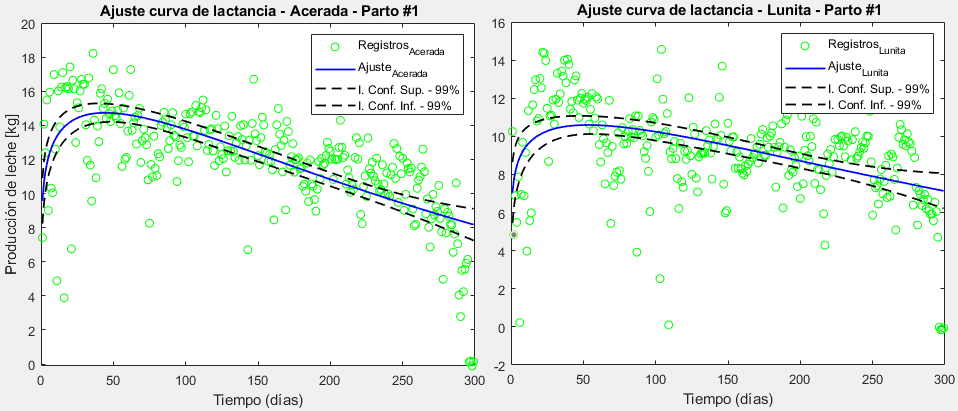
\includegraphics[scale=0.64]{img/lev1p1.png}
	 \end{center}
	 \caption{Ajustes de curvas de lactancia para Acerada y Lunita, Parto\#1.  \label{levenberg1}}
\end{figure}

De los resultados obtenidos por el método anterior, se pueden estimar los valores de los parámetros $\alpha$, $\beta$ y $\gamma$ para cada una de las reses. Teniéndose como resultado un total de 84 parámetros usados para representas las 28 curvas de lactancia para las vacas de la tabla \ref{Nporpartos}. Este algoritmo es especialmente útil para evidenciar las ejecuciones del mismo hasta lograr la aproximación de los parámetros de interés:

\begin{figure}[H]
	 \begin{center}
	 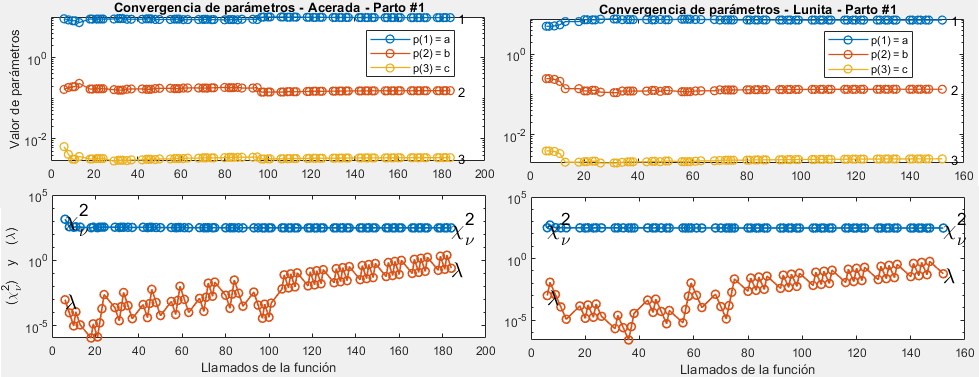
\includegraphics[scale=0.64]{img/parslev1.png}
	 \end{center}
	 \caption{Convergencia de parámetros estimados del modelo de Wood para Acerada y Lunita. \label{levenberg1}}
\end{figure}

% Feb 19 2023----- Debería tener una tabla con 84 los parámetros hallados por LM, por MIXED y por ESTOCASTICOS ?? Preguntar a Tobón

\subsection{Método de ajuste no lineal: Efectos mixtos (ME)}

Para este caso, los sujetos de estudio son las reses de cada parto y se busca estimar los parámetros de ajuste de cada vaca aún cuando el modelo plantee una solución generalizada para cada parto.


Supóngase que se realiza un ajuste no-lineal como el de Levenberg-Marquardt a las reses de cada parto, obteniéndose las figuras \ref{nlinfit1png} y \ref{nlinfitbox1png}:

\begin{figure}[H]
	 \begin{center}
	 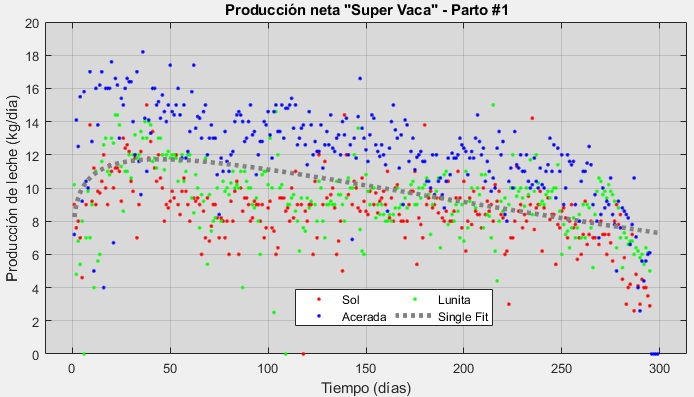
\includegraphics[scale=0.69]{img/nlinfit1spa.jpg}
	 \end{center}
	 \caption{Estimación no Lineal de parámetros generalizado del modelo de Wood para las reses del parto 1. \label{nlinfit1png}}
\end{figure}

De la figura \ref{nlinfitbox1png} se puede observar que los residuos de las reses del parto 1 se encuentran por encima o por debajo de 0, lo que indica que el modelo ha fallado en identificar los efectos específicos en el sujeto. Para lograr la identificación de los efectos específicos de cada vaca se debe hacer un ajuste individual tal y como se observa en la figura \ref{nlinfitmultiplepng}:

\begin{figure}[H]
	 \begin{center}
	 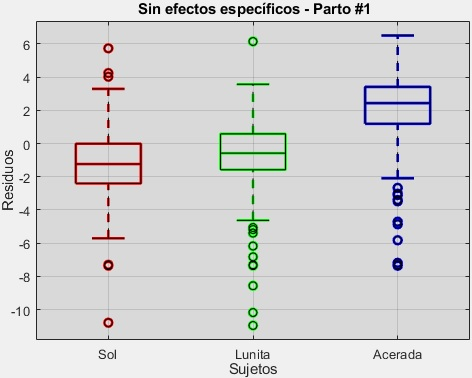
\includegraphics[scale=0.7]{img/nlinfitbox1spa.jpg}
	 \end{center}
	 \caption{Diagrama de cajas y bigotes para las reses del parto 1. \label{nlinfitbox1png}}
\end{figure}

\begin{figure}[H]
	 \begin{center}
	 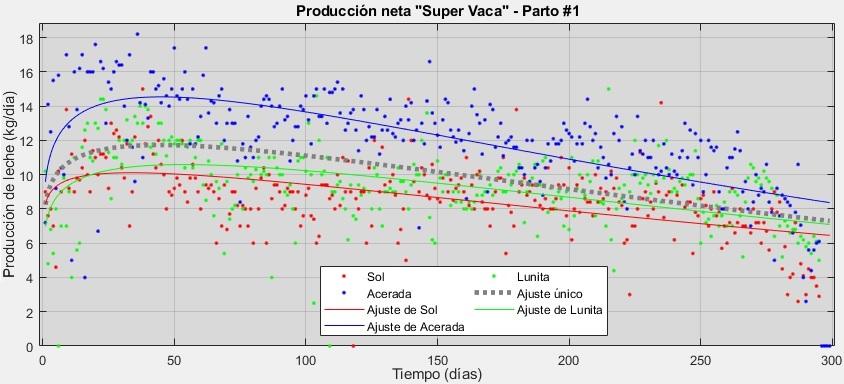
\includegraphics[scale=0.69]{img/nlinfitmultiplespa.jpg}
	 \end{center}
	 \caption{Estimación no Lineal de parámetros individualizado del modelo de Wood para las reses del parto 1. \label{nlinfitmultiplepng}}
\end{figure}

Repitiendo este proceso de comparación, se puede observar que incluso para aquellos partos que cuentan con 7 reses, la estimación individualizada permite una disminución del  error cuadrático medio concluyendo así que el ajuste para efectos específicos representa mejor ajuste que el modelo generalizado. Por otra parte, los diagramas de cajas y bigotes también muestran una mejoría notable, pues se evidencia que los residuos del ajuste tienden a estar centrados en 0, y el tamaño de las cajas disminuye a comparación del modelo anterior.

\begin{figure}[H]
	 \begin{center}
	 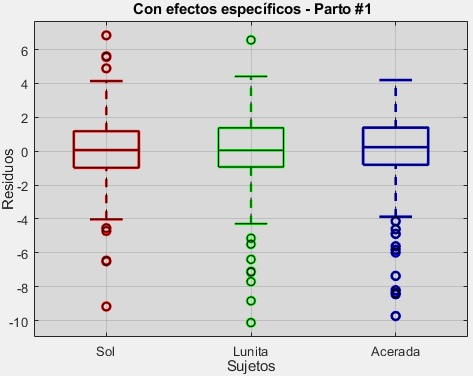
\includegraphics[scale=0.9]{img/nlinfitboxmultiplespa.jpg}
	 \end{center}
	 \caption{Diagrama de cajas y bigotes individualizado para las reses del parto 1. \label{nlinfitbox1png}}
\end{figure}

Aún cuando este ajuste ha probado tener mejores resultados que el ajuste no lineal por el método de LM, y explica con éxito las variaciones debidas a los sujetos específicos del estudio, no considera a los sujetos como representantes de una población más grande, esto es, para casos donde se tuvieran más sujetos de estudio a comparación de los existentes. El propósito de los modelos de efectos mixtos es dar cuenta de las variaciones específicas de los sujetos de manera más amplia, como efectos aleatorios que varían en torno a las medias de la población. Por tal motivo se considera pertinente realizar un análisis complementario para un ajuste no lineal con efectos mixtos aleatorios. %  mediante el uso de efectos mixtos estocásticos.
\pagebreak
% \subsection{Método de ajuste no lineal: Efectos mixtos estocásticos}
\subsection{Método de ajuste no lineal: Efectos mixtos (ME) aleatorios}

En este caso, el método de ajuste no lineal utilizado con anterioridad es cambiado por la función de ajuste no lineal de efectos mixtos ``nlmefit'', la que por defecto  asigna efectos aleatorios a todos los parámetros del modelo. También de forma predeterminada, asume una matriz sin covarianza entre los efectos aleatorios para evitar la parametrización excesiva y los problemas de convergencia relacionados.\\

De esta función, utilizada en Matlab, se pueden extraer algunos criterios adicionales que puedes complementar las decisiones tomadas en el método, como por ejemplo la reducción de los parámetros AIC y BIC. El criterio de información de Akaike (AIC) y el criterio de información bayesiano (BIC) son dos medidas de la calidad del ajuste de un modelo estadístico, que se utilizan comúnmente para seleccionar el mejor modelo entre varios modelos candidatos. En general, se prefiere un modelo con un valor más bajo de AIC o BIC, ya que esto indica que el modelo tiene una buena bondad de ajuste y una complejidad adecuada. Sin embargo, no hay un umbral fijo para considerar un modelo ``bueno'' o ``malo'' en términos de estos criterios. En cambio, se comparan los valores de AIC o BIC de varios modelos candidatos para seleccionar el mejor modelo \cite{matlabmixed}.\\

La matriz de covarianza generada para cada parto puede presentar algunos valores cercanos a 0. Este tipo de valores sugieren que los efectos aleatorios en esos parámetros pueden removerse para simplificar el modelo. Esto se logra y se justifica nuevamente al notar que los criterios AIC y BIC disminuyen nuevamente.

Para evidenciar la relación existente entre parámetros, es posible graficar las matrices de covarianza del método ``nlmefit'', en donde los valores altamente correlacionados son cercanos a 1 y los que no, son forzados a 0. Para este trabajo de grado, se obtienen las relaciones en las matrices de covarianza mostradas en la figura  \ref{covmatricespng}. Identifíquese que el modelo de Wood requiere de la estimación de 3 parámetros por lo que originalmente las matrices de correlación entre parámetros aleatorios deberían ser de dimensión 3 para todos los partos, pero como algunas correlaciones a aleatorios resultan ser cercanas a 0, esta dimensión disminuye en algunos casos, ocasionando que la complejidad de ajuste sea mucho menor. Nuevamente estos resultados son soportados por la disminución en los criterios AIC y BIC, que aunque la disminución no es considerable, es menor a la anterior y por tanto representa un mejor ajuste.\\

Finalmente, una vez ejecuta el método nuevamente y teniendo en cuenta las consideraciones mencionadas hasta este momento, se generan los parámetros $b_{i}$, encargados de entregar las predicciones de los parámetros para cada una de las reses; con lo que se procede a sumar $b_{i}$ con los estimados de efectos fijos para producir el modelo de efectos mixtos final. Este proceso se repite para cada uno de los partos mediante un bucle, pero por motivos de espacio y lectura no son mostrados a continuación. (Ver script de Matlab denominado ``AnaMixEffGenBeta.m''). Los resultados obtenidos por el modelo de efectos mixtos son contrastados con la primer estimación no lineal del método de LM y mostrados en la figura \ref{mixedfinalpng}:

\begin{figure}[H]
	 \begin{center}
	 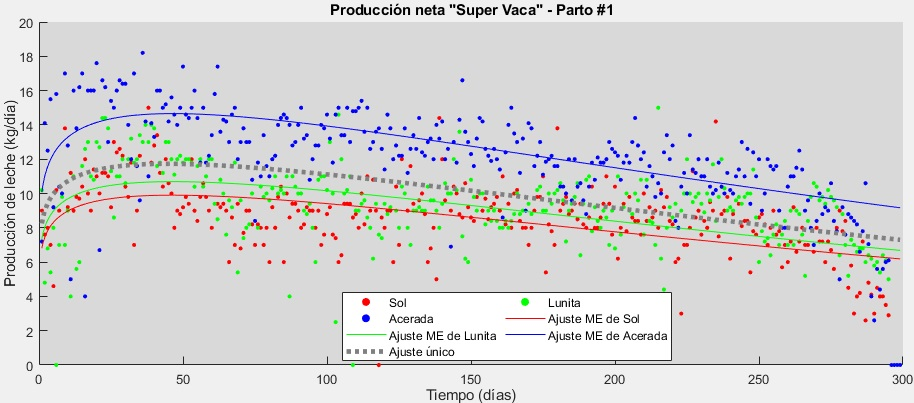
\includegraphics[scale=0.60]{img/mixedfinalspa.jpg}
	 \end{center}
	 \caption{Comparación final entre: a) Ajuste por efectos mixtos y b) Ajuste no-lineal por LM . \label{mixedfinalpng}}
\end{figure}

Adicionalmente, si no tenemos en cuenta la poca cantidad de valores atípicos existentes en los datos y evidenciados en los diagramas de cajas y bigotes; se puede establecer que la siguiente gráfica de probabilidad normal de los residuos muestra un acuerdo razonable con los supuestos del modelo sobre los errores (ver figura \ref{residprobnormpng})

\begin{figure}[H]
	 \begin{center}
	 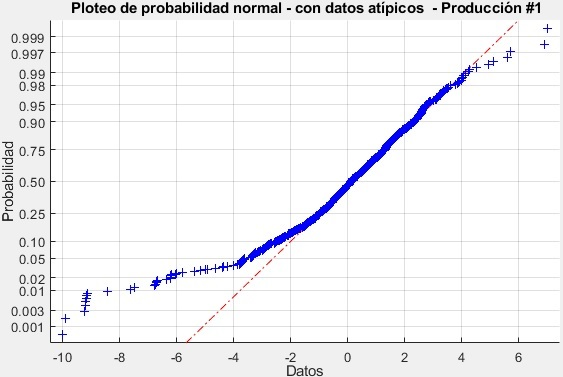
\includegraphics[scale=0.7]{img/residprobnormspa.jpg}
	 \end{center}
	 \caption{Gráfica de probabilidad normal en los residuos. Parto \#1. \label{residprobnormpng}}
\end{figure}

Cabe resaltar que este análisis es llevado a cabo para cada res y cada parto, pero por motivos de espacio y extensión de este trabajo; solo se muestran resultados del primer parto. Las demás gráficas y valores pueden ser corroborados en los scripts de Matlab y Python.

\begin{figure}[H]
	 \begin{center}
	 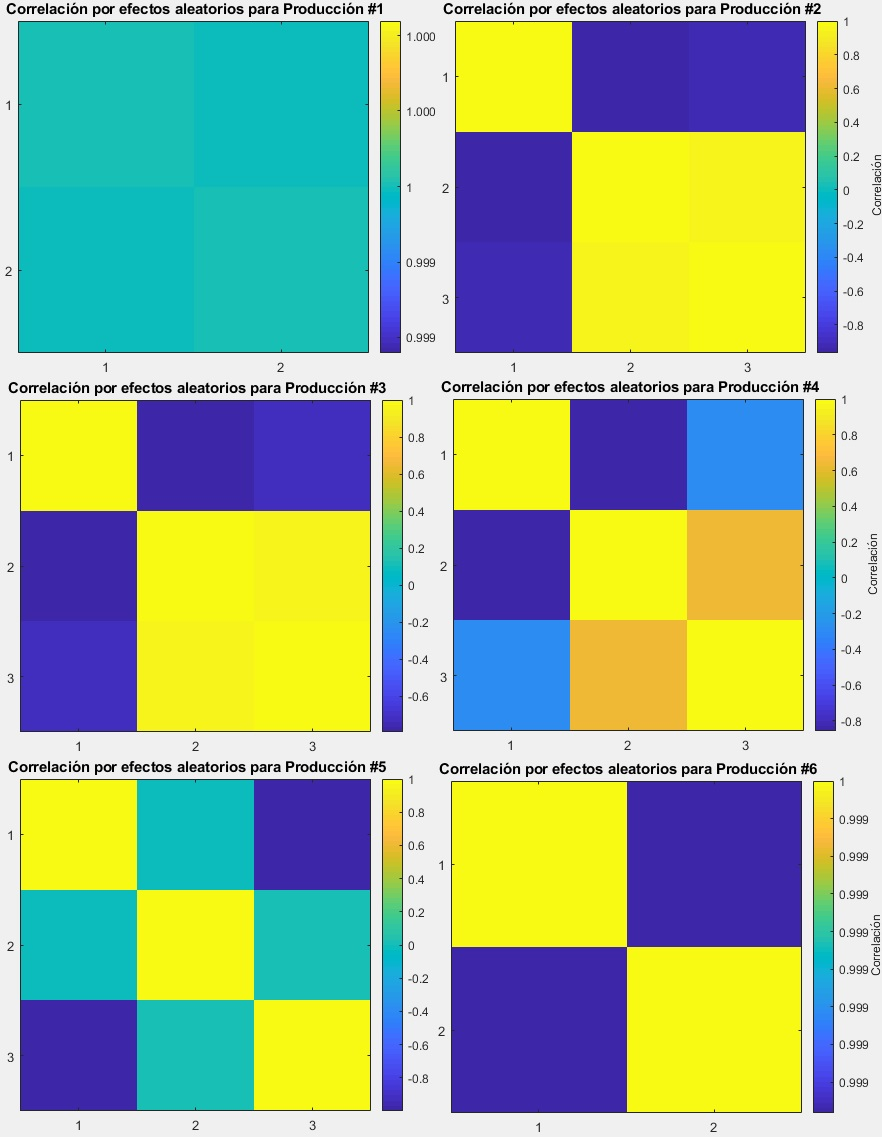
\includegraphics[scale=0.64]{img/covmatricesspa.jpg}
	 \end{center}
	 \caption{Correlación de parámetros por efectos aleatorios. \label{covmatricespng}}
\end{figure}

\pagebreak

% Please add the following required packages to your document preamble:
% \usepackage{multirow}
% \usepackage{graphicx}
% \usepackage[table,xcdraw]{xcolor}
% If you use beamer only pass "xcolor=table" option, i.e. \documentclass[xcolor=table]{beamer}
% Please add the following required packages to your document preamble:
% \usepackage{multirow}
% \usepackage{graphicx}
% \usepackage[table,xcdraw]{xcolor}
% If you use beamer only pass "xcolor=table" option, i.e. \documentclass[xcolor=table]{beamer}

% \begin{table}[]
% \centering
% \caption{Resumen de los parámetros de ajuste para cada método usado.}
% \label{tab:allparams}
% \resizebox{\textwidth}{!}{%
% \begin{tabular}{|ccc|cccccccccccccccccc|}
% \hline
% \rowcolor[HTML]{FFD9AC} 
% \multicolumn{3}{|c|}{\cellcolor[HTML]{FFD9AC}} &
%   \multicolumn{3}{c|}{\cellcolor[HTML]{FFD9AC}\textbf{EMPÍRICOS}} &
%   \multicolumn{3}{c|}{\cellcolor[HTML]{FFD9AC}\textbf{"FIT" - LM}} &
%   \multicolumn{3}{c|}{\cellcolor[HTML]{FFD9AC}\textbf{"FIT" - UNICO}} &
%   \multicolumn{3}{c|}{\cellcolor[HTML]{FFD9AC}\textbf{"FIT" - EM F}} &
%   \multicolumn{3}{c|}{\cellcolor[HTML]{FFD9AC}\textbf{"FIT" - EM A}} &
%   \multicolumn{3}{c|}{\cellcolor[HTML]{FFD9AC}\textbf{PROM}} \\ \hline
% \rowcolor[HTML]{FFD9AC} 
% \multicolumn{1}{|c|}{\cellcolor[HTML]{FFD9AC}} &
%   \multicolumn{1}{c|}{\cellcolor[HTML]{FFD9AC}} &
%   \textbf{PARS} &
%   \multicolumn{1}{c|}{\cellcolor[HTML]{FFD9AC}\textbf{a}} &
%   \multicolumn{1}{c|}{\cellcolor[HTML]{FFD9AC}\textbf{b}} &
%   \multicolumn{1}{c|}{\cellcolor[HTML]{FFD9AC}\textbf{c}} &
%   \multicolumn{1}{c|}{\cellcolor[HTML]{FFD9AC}\textbf{a}} &
%   \multicolumn{1}{c|}{\cellcolor[HTML]{FFD9AC}\textbf{b}} &
%   \multicolumn{1}{c|}{\cellcolor[HTML]{FFD9AC}\textbf{c}} &
%   \multicolumn{1}{c|}{\cellcolor[HTML]{FFD9AC}\textbf{a}} &
%   \multicolumn{1}{c|}{\cellcolor[HTML]{FFD9AC}\textbf{b}} &
%   \multicolumn{1}{c|}{\cellcolor[HTML]{FFD9AC}\textbf{c}} &
%   \multicolumn{1}{c|}{\cellcolor[HTML]{FFD9AC}\textbf{a}} &
%   \multicolumn{1}{c|}{\cellcolor[HTML]{FFD9AC}\textbf{b}} &
%   \multicolumn{1}{c|}{\cellcolor[HTML]{FFD9AC}\textbf{c}} &
%   \multicolumn{1}{c|}{\cellcolor[HTML]{FFD9AC}\textbf{a}} &
%   \multicolumn{1}{c|}{\cellcolor[HTML]{FFD9AC}\textbf{b}} &
%   \multicolumn{1}{c|}{\cellcolor[HTML]{FFD9AC}\textbf{c}} &
%   \multicolumn{1}{c|}{\cellcolor[HTML]{FFD9AC}\textbf{a}} &
%   \multicolumn{1}{c|}{\cellcolor[HTML]{FFD9AC}\textbf{b}} &
%   \textbf{c} \\ \cline{3-21} 
% \rowcolor[HTML]{FFD9AC} 
% \multicolumn{1}{|c|}{\multirow{-2}{*}{\cellcolor[HTML]{FFD9AC}\textbf{\begin{tabular}[c]{@{}c@{}}PARTO\\   P \#i\end{tabular}}}} &
%   \multicolumn{1}{c|}{\multirow{-2}{*}{\cellcolor[HTML]{FFD9AC}\textbf{N}}} &
%   \textbf{VACA} &
%   \multicolumn{18}{c|}{\cellcolor[HTML]{FFD9AC}} \\ \hline
% \multicolumn{1}{|c|}{\cellcolor[HTML]{343434}{\color[HTML]{FFFFFF} }} &
%   \multicolumn{1}{c|}{\cellcolor[HTML]{343434}{\color[HTML]{FFFFFF} }} &
%   \cellcolor[HTML]{656565}{\color[HTML]{FFFFFF} \textbf{ACER}} &
%   \multicolumn{1}{c|}{\textit{\textbf{15.500}}} &
%   \multicolumn{1}{c|}{\textit{\textbf{0.045}}} &
%   \multicolumn{1}{c|}{\textit{\textbf{0.007}}} &
%   \multicolumn{1}{c|}{\textit{\textbf{9.602}}} &
%   \multicolumn{1}{c|}{\textit{\textbf{0.153}}} &
%   \multicolumn{1}{c|}{\textit{\textbf{0.004}}} &
%   \multicolumn{1}{c|}{} &
%   \multicolumn{1}{c|}{} &
%   \multicolumn{1}{c|}{} &
%   \multicolumn{1}{c|}{\textit{\textbf{9.612}}} &
%   \multicolumn{1}{c|}{\textit{\textbf{0.147}}} &
%   \multicolumn{1}{c|}{\textit{\textbf{0.003}}} &
%   \multicolumn{1}{c|}{\textit{\textbf{10.098}}} &
%   \multicolumn{1}{c|}{\textit{\textbf{0.131}}} &
%   \multicolumn{1}{c|}{\textit{\textbf{0.003}}} &
%   \multicolumn{1}{c|}{\textit{\textbf{10.617}}} &
%   \multicolumn{1}{c|}{\textit{\textbf{0.120}}} &
%   \textit{\textbf{0.004}} \\ \cline{3-9} \cline{13-21} 
% \multicolumn{1}{|c|}{\cellcolor[HTML]{343434}{\color[HTML]{FFFFFF} }} &
%   \multicolumn{1}{c|}{\cellcolor[HTML]{343434}{\color[HTML]{FFFFFF} }} &
%   \cellcolor[HTML]{656565}{\color[HTML]{FFFFFF} \textbf{SOL}} &
%   \multicolumn{1}{c|}{\textit{\textbf{7.000}}} &
%   \multicolumn{1}{c|}{\textit{\textbf{0.210}}} &
%   \multicolumn{1}{c|}{\textit{\textbf{0.008}}} &
%   \multicolumn{1}{c|}{\textit{\textbf{7.405}}} &
%   \multicolumn{1}{c|}{\textit{\textbf{0.119}}} &
%   \multicolumn{1}{c|}{\textit{\textbf{0.003}}} &
%   \multicolumn{1}{c|}{} &
%   \multicolumn{1}{c|}{} &
%   \multicolumn{1}{c|}{} &
%   \multicolumn{1}{c|}{\textit{\textbf{8.295}}} &
%   \multicolumn{1}{c|}{\textit{\textbf{0.079}}} &
%   \multicolumn{1}{c|}{\textit{\textbf{0.002}}} &
%   \multicolumn{1}{c|}{\textit{\textbf{6.833}}} &
%   \multicolumn{1}{c|}{\textit{\textbf{0.131}}} &
%   \multicolumn{1}{c|}{\textit{\textbf{0.003}}} &
%   \multicolumn{1}{c|}{\textit{\textbf{7.561}}} &
%   \multicolumn{1}{c|}{\textit{\textbf{0.133}}} &
%   \textit{\textbf{0.004}} \\ \cline{3-9} \cline{13-21} 
% \multicolumn{1}{|c|}{\multirow{-3}{*}{\cellcolor[HTML]{343434}{\color[HTML]{FFFFFF} \textbf{P \#1}}}} &
%   \multicolumn{1}{c|}{\multirow{-3}{*}{\cellcolor[HTML]{343434}{\color[HTML]{FFFFFF} \textbf{299}}}} &
%   \cellcolor[HTML]{656565}{\color[HTML]{FFFFFF} \textbf{LUN}} &
%   \multicolumn{1}{c|}{\textit{\textbf{5.400}}} &
%   \multicolumn{1}{c|}{\textit{\textbf{0.317}}} &
%   \multicolumn{1}{c|}{\textit{\textbf{0.006}}} &
%   \multicolumn{1}{c|}{\textit{\textbf{7.067}}} &
%   \multicolumn{1}{c|}{\textit{\textbf{0.136}}} &
%   \multicolumn{1}{c|}{\textit{\textbf{0.003}}} &
%   \multicolumn{1}{c|}{\multirow{-3}{*}{\textit{\textbf{8.273}}}} &
%   \multicolumn{1}{c|}{\multirow{-3}{*}{\textit{\textbf{0.125}}}} &
%   \multicolumn{1}{c|}{\multirow{-3}{*}{\textit{\textbf{0.003}}}} &
%   \multicolumn{1}{c|}{\textit{\textbf{6.986}}} &
%   \multicolumn{1}{c|}{\textit{\textbf{0.140}}} &
%   \multicolumn{1}{c|}{\textit{\textbf{0.003}}} &
%   \multicolumn{1}{c|}{\textit{\textbf{7.375}}} &
%   \multicolumn{1}{c|}{\textit{\textbf{0.131}}} &
%   \multicolumn{1}{c|}{\textit{\textbf{0.003}}} &
%   \multicolumn{1}{c|}{\textit{\textbf{7.020}}} &
%   \multicolumn{1}{c|}{\textit{\textbf{0.170}}} &
%   \textit{\textbf{0.003}} \\ \hline
% \multicolumn{1}{|c|}{\cellcolor[HTML]{3241CB}{\color[HTML]{FFFFFF} }} &
%   \multicolumn{1}{c|}{\cellcolor[HTML]{3241CB}{\color[HTML]{FFFFFF} }} &
%   \cellcolor[HTML]{BDFFFC}\textbf{DIAN} &
%   \multicolumn{1}{c|}{\textit{\textbf{21.000}}} &
%   \multicolumn{1}{c|}{\textit{\textbf{0.080}}} &
%   \multicolumn{1}{c|}{\textit{\textbf{0.005}}} &
%   \multicolumn{1}{c|}{\textit{\textbf{15.930}}} &
%   \multicolumn{1}{c|}{\textit{\textbf{0.114}}} &
%   \multicolumn{1}{c|}{\textit{\textbf{0.004}}} &
%   \multicolumn{1}{c|}{} &
%   \multicolumn{1}{c|}{} &
%   \multicolumn{1}{c|}{} &
%   \multicolumn{1}{c|}{\textit{\textbf{16.220}}} &
%   \multicolumn{1}{c|}{\textit{\textbf{0.107}}} &
%   \multicolumn{1}{c|}{\textit{\textbf{0.004}}} &
%   \multicolumn{1}{c|}{\textit{\textbf{16.154}}} &
%   \multicolumn{1}{c|}{\textit{\textbf{0.109}}} &
%   \multicolumn{1}{c|}{\textit{\textbf{0.004}}} &
%   \multicolumn{1}{c|}{\textit{\textbf{16.303}}} &
%   \multicolumn{1}{c|}{\textit{\textbf{0.113}}} &
%   \textit{\textbf{0.014}} \\ \cline{3-9} \cline{13-21} 
% \multicolumn{1}{|c|}{\cellcolor[HTML]{3241CB}{\color[HTML]{FFFFFF} }} &
%   \multicolumn{1}{c|}{\cellcolor[HTML]{3241CB}{\color[HTML]{FFFFFF} }} &
%   \cellcolor[HTML]{BDFFFC}\textbf{GINA} &
%   \multicolumn{1}{c|}{\textit{\textbf{20.400}}} &
%   \multicolumn{1}{c|}{\textit{\textbf{0.168}}} &
%   \multicolumn{1}{c|}{\textit{\textbf{0.009}}} &
%   \multicolumn{1}{c|}{\textit{\textbf{11.950}}} &
%   \multicolumn{1}{c|}{\textit{\textbf{0.251}}} &
%   \multicolumn{1}{c|}{\textit{\textbf{0.007}}} &
%   \multicolumn{1}{c|}{} &
%   \multicolumn{1}{c|}{} &
%   \multicolumn{1}{c|}{} &
%   \multicolumn{1}{c|}{\textit{\textbf{16.059}}} &
%   \multicolumn{1}{c|}{\textit{\textbf{0.149}}} &
%   \multicolumn{1}{c|}{\textit{\textbf{0.006}}} &
%   \multicolumn{1}{c|}{\textit{\textbf{15.553}}} &
%   \multicolumn{1}{c|}{\textit{\textbf{0.158}}} &
%   \multicolumn{1}{c|}{\textit{\textbf{0.006}}} &
%   \multicolumn{1}{c|}{\textit{\textbf{15.234}}} &
%   \multicolumn{1}{c|}{\textit{\textbf{0.176}}} &
%   \textit{\textbf{0.016}} \\ \cline{3-9} \cline{13-21} 
% \multicolumn{1}{|c|}{\cellcolor[HTML]{3241CB}{\color[HTML]{FFFFFF} }} &
%   \multicolumn{1}{c|}{\cellcolor[HTML]{3241CB}{\color[HTML]{FFFFFF} }} &
%   \cellcolor[HTML]{BDFFFC}\textbf{JUAN} &
%   \multicolumn{1}{c|}{\textit{\textbf{9.400}}} &
%   \multicolumn{1}{c|}{\textit{\textbf{0.126}}} &
%   \multicolumn{1}{c|}{\textit{\textbf{0.010}}} &
%   \multicolumn{1}{c|}{\textit{\textbf{4.103}}} &
%   \multicolumn{1}{c|}{\textit{\textbf{0.317}}} &
%   \multicolumn{1}{c|}{\textit{\textbf{0.008}}} &
%   \multicolumn{1}{c|}{} &
%   \multicolumn{1}{c|}{} &
%   \multicolumn{1}{c|}{} &
%   \multicolumn{1}{c|}{\textit{\textbf{4.384}}} &
%   \multicolumn{1}{c|}{\textit{\textbf{0.282}}} &
%   \multicolumn{1}{c|}{\textit{\textbf{0.007}}} &
%   \multicolumn{1}{c|}{\textit{\textbf{5.119}}} &
%   \multicolumn{1}{c|}{\textit{\textbf{0.233}}} &
%   \multicolumn{1}{c|}{\textit{\textbf{0.007}}} &
%   \multicolumn{1}{c|}{\textit{\textbf{7.043}}} &
%   \multicolumn{1}{c|}{\textit{\textbf{0.222}}} &
%   \textit{\textbf{0.017}} \\ \cline{3-9} \cline{13-21} 
% \multicolumn{1}{|c|}{\cellcolor[HTML]{3241CB}{\color[HTML]{FFFFFF} }} &
%   \multicolumn{1}{c|}{\cellcolor[HTML]{3241CB}{\color[HTML]{FFFFFF} }} &
%   \cellcolor[HTML]{BDFFFC}\textbf{LUCI} &
%   \multicolumn{1}{c|}{\textit{\textbf{19.000}}} &
%   \multicolumn{1}{c|}{\textit{\textbf{0.028}}} &
%   \multicolumn{1}{c|}{\textit{\textbf{0.005}}} &
%   \multicolumn{1}{c|}{\textit{\textbf{13.394}}} &
%   \multicolumn{1}{c|}{\textit{\textbf{0.167}}} &
%   \multicolumn{1}{c|}{\textit{\textbf{0.007}}} &
%   \multicolumn{1}{c|}{} &
%   \multicolumn{1}{c|}{} &
%   \multicolumn{1}{c|}{} &
%   \multicolumn{1}{c|}{\textit{\textbf{13.801}}} &
%   \multicolumn{1}{c|}{\textit{\textbf{0.147}}} &
%   \multicolumn{1}{c|}{\textit{\textbf{0.006}}} &
%   \multicolumn{1}{c|}{\textit{\textbf{13.127}}} &
%   \multicolumn{1}{c|}{\textit{\textbf{0.160}}} &
%   \multicolumn{1}{c|}{\textit{\textbf{0.006}}} &
%   \multicolumn{1}{c|}{\textit{\textbf{14.306}}} &
%   \multicolumn{1}{c|}{\textit{\textbf{0.131}}} &
%   \textit{\textbf{0.015}} \\ \cline{3-9} \cline{13-21} 
% \multicolumn{1}{|c|}{\cellcolor[HTML]{3241CB}{\color[HTML]{FFFFFF} }} &
%   \multicolumn{1}{c|}{\cellcolor[HTML]{3241CB}{\color[HTML]{FFFFFF} }} &
%   \cellcolor[HTML]{BDFFFC}\textbf{PAC} &
%   \multicolumn{1}{c|}{\textit{\textbf{18.600}}} &
%   \multicolumn{1}{c|}{\textit{\textbf{0.069}}} &
%   \multicolumn{1}{c|}{\textit{\textbf{0.004}}} &
%   \multicolumn{1}{c|}{\textit{\textbf{20.167}}} &
%   \multicolumn{1}{c|}{\textit{\textbf{-0.036}}} &
%   \multicolumn{1}{c|}{\textit{\textbf{0.002}}} &
%   \multicolumn{1}{c|}{} &
%   \multicolumn{1}{c|}{} &
%   \multicolumn{1}{c|}{} &
%   \multicolumn{1}{c|}{\textit{\textbf{19.752}}} &
%   \multicolumn{1}{c|}{\textit{\textbf{-0.027}}} &
%   \multicolumn{1}{c|}{\textit{\textbf{0.002}}} &
%   \multicolumn{1}{c|}{\textit{\textbf{18.765}}} &
%   \multicolumn{1}{c|}{\textit{\textbf{-0.010}}} &
%   \multicolumn{1}{c|}{\textit{\textbf{0.002}}} &
%   \multicolumn{1}{c|}{\textit{\textbf{17.899}}} &
%   \multicolumn{1}{c|}{\textit{\textbf{0.030}}} &
%   \textit{\textbf{0.013}} \\ \cline{3-9} \cline{13-21} 
% \multicolumn{1}{|c|}{\cellcolor[HTML]{3241CB}{\color[HTML]{FFFFFF} }} &
%   \multicolumn{1}{c|}{\cellcolor[HTML]{3241CB}{\color[HTML]{FFFFFF} }} &
%   \cellcolor[HTML]{BDFFFC}\textbf{SOL} &
%   \multicolumn{1}{c|}{\textit{\textbf{16.800}}} &
%   \multicolumn{1}{c|}{\textit{\textbf{0.078}}} &
%   \multicolumn{1}{c|}{\textit{\textbf{0.008}}} &
%   \multicolumn{1}{c|}{\textit{\textbf{10.138}}} &
%   \multicolumn{1}{c|}{\textit{\textbf{0.220}}} &
%   \multicolumn{1}{c|}{\textit{\textbf{0.007}}} &
%   \multicolumn{1}{c|}{} &
%   \multicolumn{1}{c|}{} &
%   \multicolumn{1}{c|}{} &
%   \multicolumn{1}{c|}{\textit{\textbf{9.374}}} &
%   \multicolumn{1}{c|}{\textit{\textbf{0.238}}} &
%   \multicolumn{1}{c|}{\textit{\textbf{0.007}}} &
%   \multicolumn{1}{c|}{\textit{\textbf{9.673}}} &
%   \multicolumn{1}{c|}{\textit{\textbf{0.227}}} &
%   \multicolumn{1}{c|}{\textit{\textbf{0.007}}} &
%   \multicolumn{1}{c|}{\textit{\textbf{11.639}}} &
%   \multicolumn{1}{c|}{\textit{\textbf{0.184}}} &
%   \textit{\textbf{0.016}} \\ \cline{3-9} \cline{13-21} 
% \multicolumn{1}{|c|}{\multirow{-7}{*}{\cellcolor[HTML]{3241CB}{\color[HTML]{FFFFFF} \textbf{P \#2}}}} &
%   \multicolumn{1}{c|}{\multirow{-7}{*}{\cellcolor[HTML]{3241CB}{\color[HTML]{FFFFFF} \textbf{288}}}} &
%   \cellcolor[HTML]{BDFFFC}\textbf{VIV} &
%   \multicolumn{1}{c|}{\textit{\textbf{15.400}}} &
%   \multicolumn{1}{c|}{\textit{\textbf{0.094}}} &
%   \multicolumn{1}{c|}{\textit{\textbf{0.008}}} &
%   \multicolumn{1}{c|}{\textit{\textbf{6.794}}} &
%   \multicolumn{1}{c|}{\textit{\textbf{0.339}}} &
%   \multicolumn{1}{c|}{\textit{\textbf{0.007}}} &
%   \multicolumn{1}{c|}{\multirow{-7}{*}{\textit{\textbf{12.210}}}} &
%   \multicolumn{1}{c|}{\multirow{-7}{*}{\textit{\textbf{0.154}}}} &
%   \multicolumn{1}{c|}{\multirow{-7}{*}{\textit{\textbf{0.053}}}} &
%   \multicolumn{1}{c|}{\textit{\textbf{7.847}}} &
%   \multicolumn{1}{c|}{\textit{\textbf{0.290}}} &
%   \multicolumn{1}{c|}{\textit{\textbf{0.007}}} &
%   \multicolumn{1}{c|}{\textit{\textbf{8.830}}} &
%   \multicolumn{1}{c|}{\textit{\textbf{0.256}}} &
%   \multicolumn{1}{c|}{\textit{\textbf{0.006}}} &
%   \multicolumn{1}{c|}{\textit{\textbf{10.216}}} &
%   \multicolumn{1}{c|}{\textit{\textbf{0.226}}} &
%   \textit{\textbf{0.016}} \\ \hline
% \multicolumn{1}{|c|}{\cellcolor[HTML]{32CB00}} &
%   \multicolumn{1}{c|}{\cellcolor[HTML]{32CB00}} &
%   \cellcolor[HTML]{AAFF85}\textbf{FER} &
%   \multicolumn{1}{c|}{\textit{\textbf{21.000}}} &
%   \multicolumn{1}{c|}{\textit{\textbf{0.101}}} &
%   \multicolumn{1}{c|}{\textit{\textbf{0.006}}} &
%   \multicolumn{1}{c|}{\textit{\textbf{19.729}}} &
%   \multicolumn{1}{c|}{\textit{\textbf{0.064}}} &
%   \multicolumn{1}{c|}{\textit{\textbf{0.003}}} &
%   \multicolumn{1}{c|}{} &
%   \multicolumn{1}{c|}{} &
%   \multicolumn{1}{c|}{} &
%   \multicolumn{1}{c|}{\textit{\textbf{20.217}}} &
%   \multicolumn{1}{c|}{\textit{\textbf{0.052}}} &
%   \multicolumn{1}{c|}{\textit{\textbf{0.003}}} &
%   \multicolumn{1}{c|}{\textit{\textbf{19.466}}} &
%   \multicolumn{1}{c|}{\textit{\textbf{0.067}}} &
%   \multicolumn{1}{c|}{\textit{\textbf{0.003}}} &
%   \multicolumn{1}{c|}{\textit{\textbf{18.825}}} &
%   \multicolumn{1}{c|}{\textit{\textbf{0.086}}} &
%   \textit{\textbf{0.004}} \\ \cline{3-9} \cline{13-21} 
% \multicolumn{1}{|c|}{\cellcolor[HTML]{32CB00}} &
%   \multicolumn{1}{c|}{\cellcolor[HTML]{32CB00}} &
%   \cellcolor[HTML]{AAFF85}\textbf{GPA} &
%   \multicolumn{1}{c|}{\textit{\textbf{22.000}}} &
%   \multicolumn{1}{c|}{\textit{\textbf{0.099}}} &
%   \multicolumn{1}{c|}{\textit{\textbf{0.005}}} &
%   \multicolumn{1}{c|}{\textit{\textbf{15.206}}} &
%   \multicolumn{1}{c|}{\textit{\textbf{0.148}}} &
%   \multicolumn{1}{c|}{\textit{\textbf{0.004}}} &
%   \multicolumn{1}{c|}{} &
%   \multicolumn{1}{c|}{} &
%   \multicolumn{1}{c|}{} &
%   \multicolumn{1}{c|}{\textit{\textbf{15.638}}} &
%   \multicolumn{1}{c|}{\textit{\textbf{0.132}}} &
%   \multicolumn{1}{c|}{\textit{\textbf{0.004}}} &
%   \multicolumn{1}{c|}{\textit{\textbf{15.506}}} &
%   \multicolumn{1}{c|}{\textit{\textbf{0.136}}} &
%   \multicolumn{1}{c|}{\textit{\textbf{0.004}}} &
%   \multicolumn{1}{c|}{\textit{\textbf{16.412}}} &
%   \multicolumn{1}{c|}{\textit{\textbf{0.132}}} &
%   \textit{\textbf{0.004}} \\ \cline{3-9} \cline{13-21} 
% \multicolumn{1}{|c|}{\cellcolor[HTML]{32CB00}} &
%   \multicolumn{1}{c|}{\cellcolor[HTML]{32CB00}} &
%   \cellcolor[HTML]{AAFF85}\textbf{JUAN} &
%   \multicolumn{1}{c|}{\textit{\textbf{11.000}}} &
%   \multicolumn{1}{c|}{\textit{\textbf{0.208}}} &
%   \multicolumn{1}{c|}{\textit{\textbf{0.007}}} &
%   \multicolumn{1}{c|}{\textit{\textbf{9.445}}} &
%   \multicolumn{1}{c|}{\textit{\textbf{0.203}}} &
%   \multicolumn{1}{c|}{\textit{\textbf{0.004}}} &
%   \multicolumn{1}{c|}{} &
%   \multicolumn{1}{c|}{} &
%   \multicolumn{1}{c|}{} &
%   \multicolumn{1}{c|}{\textit{\textbf{9.485}}} &
%   \multicolumn{1}{c|}{\textit{\textbf{0.202}}} &
%   \multicolumn{1}{c|}{\textit{\textbf{0.004}}} &
%   \multicolumn{1}{c|}{\textit{\textbf{9.907}}} &
%   \multicolumn{1}{c|}{\textit{\textbf{0.190}}} &
%   \multicolumn{1}{c|}{\textit{\textbf{0.004}}} &
%   \multicolumn{1}{c|}{\textit{\textbf{10.710}}} &
%   \multicolumn{1}{c|}{\textit{\textbf{0.190}}} &
%   \textit{\textbf{0.005}} \\ \cline{3-9} \cline{13-21} 
% \multicolumn{1}{|c|}{\cellcolor[HTML]{32CB00}} &
%   \multicolumn{1}{c|}{\cellcolor[HTML]{32CB00}} &
%   \cellcolor[HTML]{AAFF85}\textbf{LETI} &
%   \multicolumn{1}{c|}{\textit{\textbf{16.200}}} &
%   \multicolumn{1}{c|}{\textit{\textbf{0.116}}} &
%   \multicolumn{1}{c|}{\textit{\textbf{0.008}}} &
%   \multicolumn{1}{c|}{\textit{\textbf{15.388}}} &
%   \multicolumn{1}{c|}{\textit{\textbf{0.098}}} &
%   \multicolumn{1}{c|}{\textit{\textbf{0.004}}} &
%   \multicolumn{1}{c|}{} &
%   \multicolumn{1}{c|}{} &
%   \multicolumn{1}{c|}{} &
%   \multicolumn{1}{c|}{\textit{\textbf{16.645}}} &
%   \multicolumn{1}{c|}{\textit{\textbf{0.069}}} &
%   \multicolumn{1}{c|}{\textit{\textbf{0.003}}} &
%   \multicolumn{1}{c|}{\textit{\textbf{16.298}}} &
%   \multicolumn{1}{c|}{\textit{\textbf{0.073}}} &
%   \multicolumn{1}{c|}{\textit{\textbf{0.004}}} &
%   \multicolumn{1}{c|}{\textit{\textbf{15.648}}} &
%   \multicolumn{1}{c|}{\textit{\textbf{0.100}}} &
%   \textit{\textbf{0.005}} \\ \cline{3-9} \cline{13-21} 
% \multicolumn{1}{|c|}{\cellcolor[HTML]{32CB00}} &
%   \multicolumn{1}{c|}{\cellcolor[HTML]{32CB00}} &
%   \cellcolor[HTML]{AAFF85}\textbf{MART} &
%   \multicolumn{1}{c|}{\textit{\textbf{10.800}}} &
%   \multicolumn{1}{c|}{\textit{\textbf{0.283}}} &
%   \multicolumn{1}{c|}{\textit{\textbf{0.007}}} &
%   \multicolumn{1}{c|}{\textit{\textbf{6.613}}} &
%   \multicolumn{1}{c|}{\textit{\textbf{0.392}}} &
%   \multicolumn{1}{c|}{\textit{\textbf{0.006}}} &
%   \multicolumn{1}{c|}{} &
%   \multicolumn{1}{c|}{} &
%   \multicolumn{1}{c|}{} &
%   \multicolumn{1}{c|}{\textit{\textbf{6.516}}} &
%   \multicolumn{1}{c|}{\textit{\textbf{0.396}}} &
%   \multicolumn{1}{c|}{\textit{\textbf{0.006}}} &
%   \multicolumn{1}{c|}{\textit{\textbf{7.084}}} &
%   \multicolumn{1}{c|}{\textit{\textbf{0.371}}} &
%   \multicolumn{1}{c|}{\textit{\textbf{0.006}}} &
%   \multicolumn{1}{c|}{\textit{\textbf{8.945}}} &
%   \multicolumn{1}{c|}{\textit{\textbf{0.318}}} &
%   \textit{\textbf{0.006}} \\ \cline{3-9} \cline{13-21} 
% \multicolumn{1}{|c|}{\cellcolor[HTML]{32CB00}} &
%   \multicolumn{1}{c|}{\cellcolor[HTML]{32CB00}} &
%   \cellcolor[HTML]{AAFF85}\textbf{MOR} &
%   \multicolumn{1}{c|}{\textit{\textbf{22.000}}} &
%   \multicolumn{1}{c|}{\textit{\textbf{0.157}}} &
%   \multicolumn{1}{c|}{\textit{\textbf{0.009}}} &
%   \multicolumn{1}{c|}{\textit{\textbf{19.921}}} &
%   \multicolumn{1}{c|}{\textit{\textbf{0.108}}} &
%   \multicolumn{1}{c|}{\textit{\textbf{0.004}}} &
%   \multicolumn{1}{c|}{} &
%   \multicolumn{1}{c|}{} &
%   \multicolumn{1}{c|}{} &
%   \multicolumn{1}{c|}{\textit{\textbf{20.858}}} &
%   \multicolumn{1}{c|}{\textit{\textbf{0.092}}} &
%   \multicolumn{1}{c|}{\textit{\textbf{0.004}}} &
%   \multicolumn{1}{c|}{\textit{\textbf{20.353}}} &
%   \multicolumn{1}{c|}{\textit{\textbf{0.096}}} &
%   \multicolumn{1}{c|}{\textit{\textbf{0.004}}} &
%   \multicolumn{1}{c|}{\textit{\textbf{19.369}}} &
%   \multicolumn{1}{c|}{\textit{\textbf{0.120}}} &
%   \textit{\textbf{0.005}} \\ \cline{3-9} \cline{13-21} 
% \multicolumn{1}{|c|}{\multirow{-7}{*}{\cellcolor[HTML]{32CB00}\textbf{P \#3}}} &
%   \multicolumn{1}{c|}{\multirow{-7}{*}{\cellcolor[HTML]{32CB00}\textbf{309}}} &
%   \cellcolor[HTML]{AAFF85}\textbf{SOL} &
%   \multicolumn{1}{c|}{\textit{\textbf{16.000}}} &
%   \multicolumn{1}{c|}{\textit{\textbf{0.064}}} &
%   \multicolumn{1}{c|}{\textit{\textbf{0.006}}} &
%   \multicolumn{1}{c|}{\textit{\textbf{12.511}}} &
%   \multicolumn{1}{c|}{\textit{\textbf{0.058}}} &
%   \multicolumn{1}{c|}{\textit{\textbf{0.003}}} &
%   \multicolumn{1}{c|}{\multirow{-7}{*}{\textit{\textbf{13.711}}}} &
%   \multicolumn{1}{c|}{\multirow{-7}{*}{\textit{\textbf{0.146}}}} &
%   \multicolumn{1}{c|}{\multirow{-7}{*}{\textit{\textbf{0.004}}}} &
%   \multicolumn{1}{c|}{\textit{\textbf{12.452}}} &
%   \multicolumn{1}{c|}{\textit{\textbf{0.059}}} &
%   \multicolumn{1}{c|}{\textit{\textbf{0.003}}} &
%   \multicolumn{1}{c|}{\textit{\textbf{12.282}}} &
%   \multicolumn{1}{c|}{\textit{\textbf{0.064}}} &
%   \multicolumn{1}{c|}{\textit{\textbf{0.003}}} &
%   \multicolumn{1}{c|}{\textit{\textbf{13.391}}} &
%   \multicolumn{1}{c|}{\textit{\textbf{0.078}}} &
%   \textit{\textbf{0.004}} \\ \hline
% \multicolumn{1}{|c|}{\cellcolor[HTML]{FFFE65}} &
%   \multicolumn{1}{c|}{\cellcolor[HTML]{FFFE65}} &
%   \cellcolor[HTML]{FFFFC7}\textbf{CENT} &
%   \multicolumn{1}{c|}{\textit{\textbf{6.600}}} &
%   \multicolumn{1}{c|}{\textit{\textbf{0.211}}} &
%   \multicolumn{1}{c|}{\textit{\textbf{0.008}}} &
%   \multicolumn{1}{c|}{\textit{\textbf{4.030}}} &
%   \multicolumn{1}{c|}{\textit{\textbf{0.375}}} &
%   \multicolumn{1}{c|}{\textit{\textbf{0.005}}} &
%   \multicolumn{1}{c|}{} &
%   \multicolumn{1}{c|}{} &
%   \multicolumn{1}{c|}{} &
%   \multicolumn{1}{c|}{\textit{\textbf{4.908}}} &
%   \multicolumn{1}{c|}{\textit{\textbf{0.314}}} &
%   \multicolumn{1}{c|}{\textit{\textbf{0.004}}} &
%   \multicolumn{1}{c|}{\textit{\textbf{5.959}}} &
%   \multicolumn{1}{c|}{\textit{\textbf{0.259}}} &
%   \multicolumn{1}{c|}{\textit{\textbf{0.004}}} &
%   \multicolumn{1}{c|}{\textit{\textbf{6.205}}} &
%   \multicolumn{1}{c|}{\textit{\textbf{0.261}}} &
%   \textit{\textbf{0.005}} \\ \cline{3-9} \cline{13-21} 
% \multicolumn{1}{|c|}{\cellcolor[HTML]{FFFE65}} &
%   \multicolumn{1}{c|}{\cellcolor[HTML]{FFFE65}} &
%   \cellcolor[HTML]{FFFFC7}\textbf{DIAN} &
%   \multicolumn{1}{c|}{\textit{\textbf{11.400}}} &
%   \multicolumn{1}{c|}{\textit{\textbf{0.106}}} &
%   \multicolumn{1}{c|}{\textit{\textbf{0.005}}} &
%   \multicolumn{1}{c|}{\textit{\textbf{10.448}}} &
%   \multicolumn{1}{c|}{\textit{\textbf{0.073}}} &
%   \multicolumn{1}{c|}{\textit{\textbf{0.003}}} &
%   \multicolumn{1}{c|}{} &
%   \multicolumn{1}{c|}{} &
%   \multicolumn{1}{c|}{} &
%   \multicolumn{1}{c|}{\textit{\textbf{10.658}}} &
%   \multicolumn{1}{c|}{\textit{\textbf{0.067}}} &
%   \multicolumn{1}{c|}{\textit{\textbf{0.002}}} &
%   \multicolumn{1}{c|}{\textit{\textbf{9.965}}} &
%   \multicolumn{1}{c|}{\textit{\textbf{0.090}}} &
%   \multicolumn{1}{c|}{\textit{\textbf{0.003}}} &
%   \multicolumn{1}{c|}{\textit{\textbf{10.400}}} &
%   \multicolumn{1}{c|}{\textit{\textbf{0.096}}} &
%   \textit{\textbf{0.003}} \\ \cline{3-9} \cline{13-21} 
% \multicolumn{1}{|c|}{\cellcolor[HTML]{FFFE65}} &
%   \multicolumn{1}{c|}{\cellcolor[HTML]{FFFE65}} &
%   \cellcolor[HTML]{FFFFC7}\textbf{LETI} &
%   \multicolumn{1}{c|}{\textit{\textbf{15.000}}} &
%   \multicolumn{1}{c|}{\textit{\textbf{0.089}}} &
%   \multicolumn{1}{c|}{\textit{\textbf{0.007}}} &
%   \multicolumn{1}{c|}{\textit{\textbf{11.952}}} &
%   \multicolumn{1}{c|}{\textit{\textbf{0.073}}} &
%   \multicolumn{1}{c|}{\textit{\textbf{0.003}}} &
%   \multicolumn{1}{c|}{} &
%   \multicolumn{1}{c|}{} &
%   \multicolumn{1}{c|}{} &
%   \multicolumn{1}{c|}{\textit{\textbf{12.857}}} &
%   \multicolumn{1}{c|}{\textit{\textbf{0.043}}} &
%   \multicolumn{1}{c|}{\textit{\textbf{0.003}}} &
%   \multicolumn{1}{c|}{\textit{\textbf{11.721}}} &
%   \multicolumn{1}{c|}{\textit{\textbf{0.073}}} &
%   \multicolumn{1}{c|}{\textit{\textbf{0.030}}} &
%   \multicolumn{1}{c|}{\textit{\textbf{12.212}}} &
%   \multicolumn{1}{c|}{\textit{\textbf{0.084}}} &
%   \textit{\textbf{0.009}} \\ \cline{3-9} \cline{13-21} 
% \multicolumn{1}{|c|}{\cellcolor[HTML]{FFFE65}} &
%   \multicolumn{1}{c|}{\cellcolor[HTML]{FFFE65}} &
%   \cellcolor[HTML]{FFFFC7}\textbf{MOR} &
%   \multicolumn{1}{c|}{\textit{\textbf{15.300}}} &
%   \multicolumn{1}{c|}{\textit{\textbf{0.077}}} &
%   \multicolumn{1}{c|}{\textit{\textbf{0.004}}} &
%   \multicolumn{1}{c|}{\textit{\textbf{12.251}}} &
%   \multicolumn{1}{c|}{\textit{\textbf{0.124}}} &
%   \multicolumn{1}{c|}{\textit{\textbf{0.005}}} &
%   \multicolumn{1}{c|}{} &
%   \multicolumn{1}{c|}{} &
%   \multicolumn{1}{c|}{} &
%   \multicolumn{1}{c|}{\textit{\textbf{13.101}}} &
%   \multicolumn{1}{c|}{\textit{\textbf{0.095}}} &
%   \multicolumn{1}{c|}{\textit{\textbf{0.004}}} &
%   \multicolumn{1}{c|}{\textit{\textbf{12.301}}} &
%   \multicolumn{1}{c|}{\textit{\textbf{0.115}}} &
%   \multicolumn{1}{c|}{\textit{\textbf{0.004}}} &
%   \multicolumn{1}{c|}{\textit{\textbf{12.497}}} &
%   \multicolumn{1}{c|}{\textit{\textbf{0.111}}} &
%   \textit{\textbf{0.004}} \\ \cline{3-9} \cline{13-21} 
% \multicolumn{1}{|c|}{\cellcolor[HTML]{FFFE65}} &
%   \multicolumn{1}{c|}{\cellcolor[HTML]{FFFE65}} &
%   \cellcolor[HTML]{FFFFC7}\textbf{MUC} &
%   \multicolumn{1}{c|}{\textit{\textbf{16.200}}} &
%   \multicolumn{1}{c|}{\textit{\textbf{0.088}}} &
%   \multicolumn{1}{c|}{\textit{\textbf{0.006}}} &
%   \multicolumn{1}{c|}{\textit{\textbf{12.259}}} &
%   \multicolumn{1}{c|}{\textit{\textbf{0.182}}} &
%   \multicolumn{1}{c|}{\textit{\textbf{0.007}}} &
%   \multicolumn{1}{c|}{} &
%   \multicolumn{1}{c|}{} &
%   \multicolumn{1}{c|}{} &
%   \multicolumn{1}{c|}{\textit{\textbf{13.138}}} &
%   \multicolumn{1}{c|}{\textit{\textbf{0.155}}} &
%   \multicolumn{1}{c|}{\textit{\textbf{0.006}}} &
%   \multicolumn{1}{c|}{\textit{\textbf{12.708}}} &
%   \multicolumn{1}{c|}{\textit{\textbf{0.164}}} &
%   \multicolumn{1}{c|}{\textit{\textbf{0.006}}} &
%   \multicolumn{1}{c|}{\textit{\textbf{12.767}}} &
%   \multicolumn{1}{c|}{\textit{\textbf{0.146}}} &
%   \textit{\textbf{0.006}} \\ \cline{3-9} \cline{13-21} 
% \multicolumn{1}{|c|}{\cellcolor[HTML]{FFFE65}} &
%   \multicolumn{1}{c|}{\cellcolor[HTML]{FFFE65}} &
%   \cellcolor[HTML]{FFFFC7}\textbf{SOR} &
%   \multicolumn{1}{c|}{\textit{\textbf{4.800}}} &
%   \multicolumn{1}{c|}{\textit{\textbf{0.311}}} &
%   \multicolumn{1}{c|}{\textit{\textbf{0.010}}} &
%   \multicolumn{1}{c|}{\textit{\textbf{5.386}}} &
%   \multicolumn{1}{c|}{\textit{\textbf{0.262}}} &
%   \multicolumn{1}{c|}{\textit{\textbf{0.007}}} &
%   \multicolumn{1}{c|}{} &
%   \multicolumn{1}{c|}{} &
%   \multicolumn{1}{c|}{} &
%   \multicolumn{1}{c|}{\textit{\textbf{5.404}}} &
%   \multicolumn{1}{c|}{\textit{\textbf{0.263}}} &
%   \multicolumn{1}{c|}{\textit{\textbf{0.007}}} &
%   \multicolumn{1}{c|}{\textit{\textbf{6.297}}} &
%   \multicolumn{1}{c|}{\textit{\textbf{0.209}}} &
%   \multicolumn{1}{c|}{\textit{\textbf{0.006}}} &
%   \multicolumn{1}{c|}{\textit{\textbf{6.283}}} &
%   \multicolumn{1}{c|}{\textit{\textbf{0.238}}} &
%   \textit{\textbf{0.007}} \\ \cline{3-9} \cline{13-21} 
% \multicolumn{1}{|c|}{\multirow{-7}{*}{\cellcolor[HTML]{FFFE65}\textbf{P \#4}}} &
%   \multicolumn{1}{c|}{\multirow{-7}{*}{\cellcolor[HTML]{FFFE65}\textbf{274}}} &
%   \cellcolor[HTML]{FFFFC7}\textbf{VIV} &
%   \multicolumn{1}{c|}{\textit{\textbf{12.200}}} &
%   \multicolumn{1}{c|}{\textit{\textbf{0.138}}} &
%   \multicolumn{1}{c|}{\textit{\textbf{0.005}}} &
%   \multicolumn{1}{c|}{\textit{\textbf{7.032}}} &
%   \multicolumn{1}{c|}{\textit{\textbf{0.210}}} &
%   \multicolumn{1}{c|}{\textit{\textbf{0.004}}} &
%   \multicolumn{1}{c|}{\multirow{-7}{*}{\textit{\textbf{9.530}}}} &
%   \multicolumn{1}{c|}{\multirow{-7}{*}{\textit{\textbf{0.144}}}} &
%   \multicolumn{1}{c|}{\multirow{-7}{*}{\textit{\textbf{0.004}}}} &
%   \multicolumn{1}{c|}{\textit{\textbf{6.831}}} &
%   \multicolumn{1}{c|}{\textit{\textbf{0.208}}} &
%   \multicolumn{1}{c|}{\textit{\textbf{0.004}}} &
%   \multicolumn{1}{c|}{\textit{\textbf{7.370}}} &
%   \multicolumn{1}{c|}{\textit{\textbf{0.186}}} &
%   \multicolumn{1}{c|}{\textit{\textbf{0.004}}} &
%   \multicolumn{1}{c|}{\textit{\textbf{8.592}}} &
%   \multicolumn{1}{c|}{\textit{\textbf{0.177}}} &
%   \textit{\textbf{0.004}} \\ \hline
% \multicolumn{1}{|c|}{\cellcolor[HTML]{D34444}} &
%   \multicolumn{1}{c|}{\cellcolor[HTML]{D34444}} &
%   \cellcolor[HTML]{FFCCC9}\textbf{GPA} &
%   \multicolumn{1}{c|}{\textit{\textbf{11.000}}} &
%   \multicolumn{1}{c|}{\textit{\textbf{0.169}}} &
%   \multicolumn{1}{c|}{\textit{\textbf{0.009}}} &
%   \multicolumn{1}{c|}{\textit{\textbf{1.619}}} &
%   \multicolumn{1}{c|}{\textit{\textbf{0.688}}} &
%   \multicolumn{1}{c|}{\textit{\textbf{0.009}}} &
%   \multicolumn{1}{c|}{} &
%   \multicolumn{1}{c|}{} &
%   \multicolumn{1}{c|}{} &
%   \multicolumn{1}{c|}{\textit{\textbf{1.531}}} &
%   \multicolumn{1}{c|}{\textit{\textbf{0.705}}} &
%   \multicolumn{1}{c|}{\textit{\textbf{0.009}}} &
%   \multicolumn{1}{c|}{\textit{\textbf{1.670}}} &
%   \multicolumn{1}{c|}{\textit{\textbf{0.679}}} &
%   \multicolumn{1}{c|}{\textit{\textbf{0.009}}} &
%   \multicolumn{1}{c|}{\textit{\textbf{4.013}}} &
%   \multicolumn{1}{c|}{\textit{\textbf{0.533}}} &
%   \textit{\textbf{0.009}} \\ \cline{3-9} \cline{13-21} 
% \multicolumn{1}{|c|}{\multirow{-2}{*}{\cellcolor[HTML]{D34444}\textbf{P \#5}}} &
%   \multicolumn{1}{c|}{\multirow{-2}{*}{\cellcolor[HTML]{D34444}\textbf{298}}} &
%   \cellcolor[HTML]{FFCCC9}\textbf{ANDRE} &
%   \multicolumn{1}{c|}{\textit{\textbf{8.600}}} &
%   \multicolumn{1}{c|}{\textit{\textbf{0.258}}} &
%   \multicolumn{1}{c|}{\textit{\textbf{0.008}}} &
%   \multicolumn{1}{c|}{\textit{\textbf{9.473}}} &
%   \multicolumn{1}{c|}{\textit{\textbf{0.213}}} &
%   \multicolumn{1}{c|}{\textit{\textbf{0.005}}} &
%   \multicolumn{1}{c|}{\multirow{-2}{*}{\textit{\textbf{4.246}}}} &
%   \multicolumn{1}{c|}{\multirow{-2}{*}{\textit{\textbf{0.425}}}} &
%   \multicolumn{1}{c|}{\multirow{-2}{*}{\textit{\textbf{0.007}}}} &
%   \multicolumn{1}{c|}{\textit{\textbf{9.881}}} &
%   \multicolumn{1}{c|}{\textit{\textbf{0.193}}} &
%   \multicolumn{1}{c|}{\textit{\textbf{0.004}}} &
%   \multicolumn{1}{c|}{\textit{\textbf{9.371}}} &
%   \multicolumn{1}{c|}{\textit{\textbf{0.210}}} &
%   \multicolumn{1}{c|}{\textit{\textbf{0.005}}} &
%   \multicolumn{1}{c|}{\textit{\textbf{8.314}}} &
%   \multicolumn{1}{c|}{\textit{\textbf{0.260}}} &
%   \textit{\textbf{0.006}} \\ \hline
% \multicolumn{1}{|c|}{\cellcolor[HTML]{6665CD}} &
%   \multicolumn{1}{c|}{\cellcolor[HTML]{6665CD}} &
%   \cellcolor[HTML]{CBCEFB}\textbf{GPA} &
%   \multicolumn{1}{c|}{\textit{\textbf{13.000}}} &
%   \multicolumn{1}{c|}{\textit{\textbf{0.173}}} &
%   \multicolumn{1}{c|}{\textit{\textbf{0.005}}} &
%   \multicolumn{1}{c|}{\textit{\textbf{14.928}}} &
%   \multicolumn{1}{c|}{\textit{\textbf{0.149}}} &
%   \multicolumn{1}{c|}{\textit{\textbf{0.004}}} &
%   \multicolumn{1}{c|}{} &
%   \multicolumn{1}{c|}{} &
%   \multicolumn{1}{c|}{} &
%   \multicolumn{1}{c|}{\textit{\textbf{14.977}}} &
%   \multicolumn{1}{c|}{\textit{\textbf{0.146}}} &
%   \multicolumn{1}{c|}{\textit{\textbf{0.004}}} &
%   \multicolumn{1}{c|}{\textit{\textbf{15.118}}} &
%   \multicolumn{1}{c|}{\textit{\textbf{0.136}}} &
%   \multicolumn{1}{c|}{\textit{\textbf{0.004}}} &
%   \multicolumn{1}{c|}{\textit{\textbf{14.628}}} &
%   \multicolumn{1}{c|}{\textit{\textbf{0.148}}} &
%   \textit{\textbf{0.004}} \\ \cline{3-9} \cline{13-21} 
% \multicolumn{1}{|c|}{\multirow{-2}{*}{\cellcolor[HTML]{6665CD}\textbf{P \#6}}} &
%   \multicolumn{1}{c|}{\multirow{-2}{*}{\cellcolor[HTML]{6665CD}\textbf{162}}} &
%   \cellcolor[HTML]{CBCEFB}\textbf{ANDRE} &
%   \multicolumn{1}{c|}{\textit{\textbf{19.200}}} &
%   \multicolumn{1}{c|}{\textit{\textbf{0.077}}} &
%   \multicolumn{1}{c|}{\textit{\textbf{0.007}}} &
%   \multicolumn{1}{c|}{\textit{\textbf{15.437}}} &
%   \multicolumn{1}{c|}{\textit{\textbf{0.118}}} &
%   \multicolumn{1}{c|}{\textit{\textbf{0.004}}} &
%   \multicolumn{1}{c|}{\multirow{-2}{*}{\textit{\textbf{15.118}}}} &
%   \multicolumn{1}{c|}{\multirow{-2}{*}{\textit{\textbf{0.136}}}} &
%   \multicolumn{1}{c|}{\multirow{-2}{*}{\textit{\textbf{0.004}}}} &
%   \multicolumn{1}{c|}{\textit{\textbf{15.247}}} &
%   \multicolumn{1}{c|}{\textit{\textbf{0.125}}} &
%   \multicolumn{1}{c|}{\textit{\textbf{0.004}}} &
%   \multicolumn{1}{c|}{\textit{\textbf{15.105}}} &
%   \multicolumn{1}{c|}{\textit{\textbf{0.136}}} &
%   \multicolumn{1}{c|}{\textit{\textbf{0.004}}} &
%   \multicolumn{1}{c|}{\textit{\textbf{16.021}}} &
%   \multicolumn{1}{c|}{\textit{\textbf{0.118}}} &
%   \textit{\textbf{0.004}} \\ \hline
% \end{tabular}%
% }
% \end{table}
\begin{figure}[H]
    \centering
    \label{tab:allparams}
    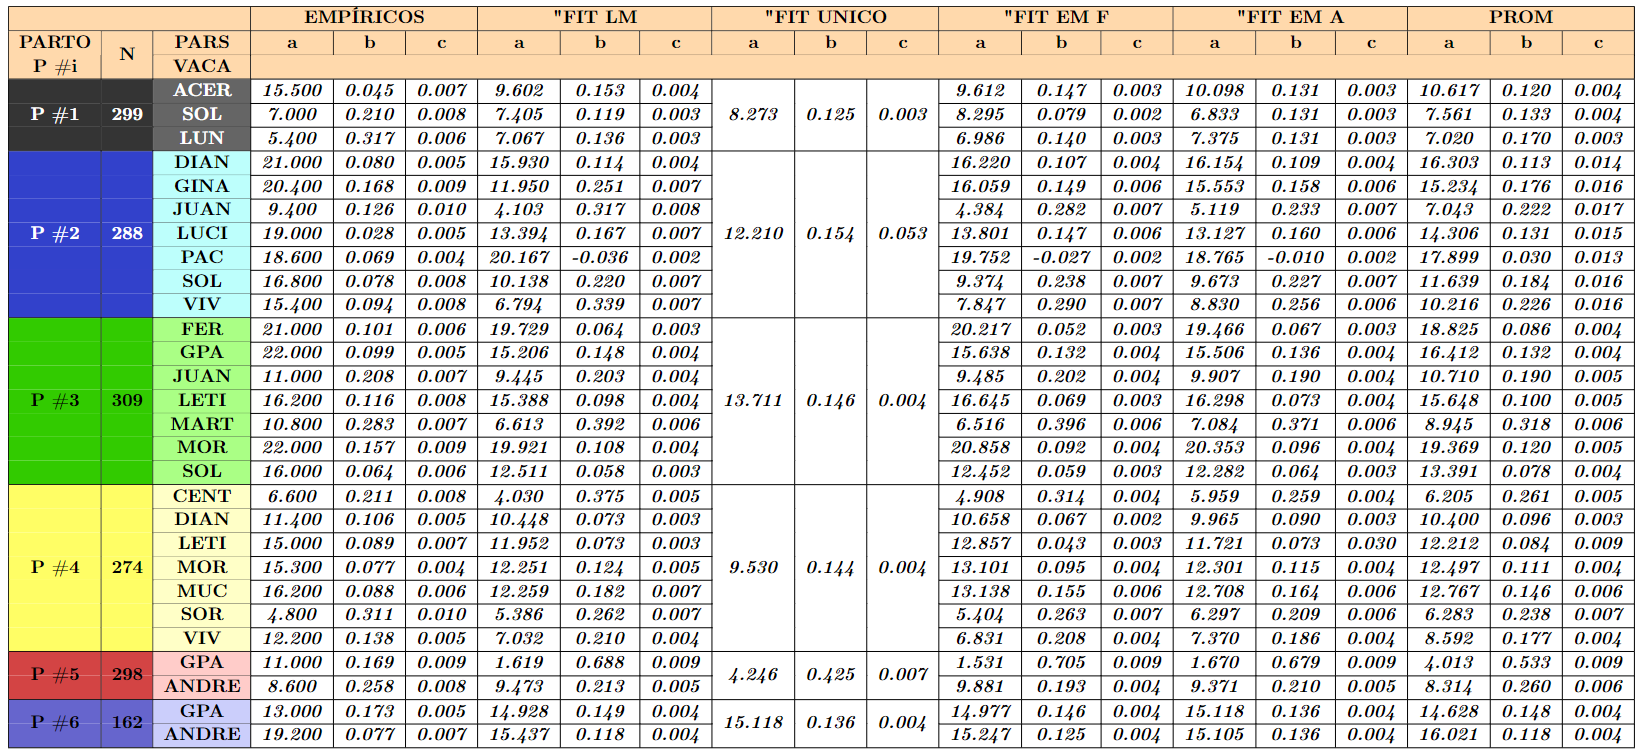
\includegraphics[angle=90,scale=0.49]{img/TabParamsFitspng.png}
    % 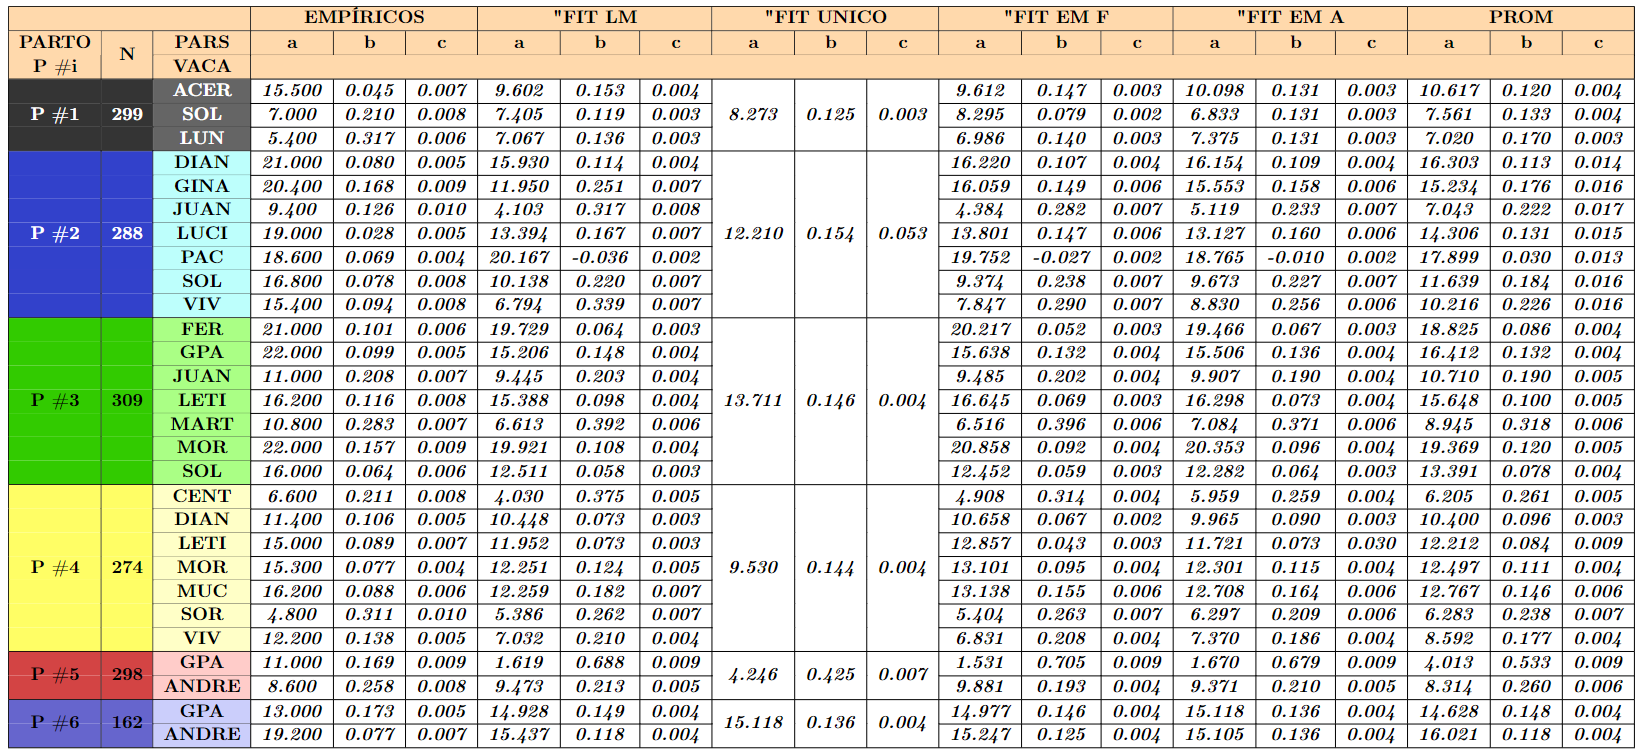
\includegraphics[angle=90, width=\textwidth, height = \paperwidth]{img/TabParamsFitspng.png}
    \caption{Resumen de los parámetros de ajuste para cada método usado}
\end{figure}

\pagebreak

%  (Tambien puedo complementar con un analisis de disminución de 0s y atipicos pero luego de tener los modelos que npi como hacer eso, y toca hacerlo para cada vaca de los partos (3+7+7+7+2+2=28 omg))


\section{Modelamiento dinámico} \label{dinamod}
\subsection{Planteamiento del modelo}

Para plantear el modelo se debe tener en cuenta los datos existentes referentes a las variables que se deseen analizar. Como primera instancia, los únicos 2 tipos de datos que se conocen son, los registros diarios de leche, para vacas de ordeño clasificadas por número de partos; y los registros de peso aproximadamente trimestral. En cuanto a otras variables como la cantidad de alimento o la cantidad de estiércol producido se pueden considerar un rango de valores aproximados entre un 1\% y 10\% respecto al peso del animal. \\

Como primera instancia, Consideraremos que las variables usadas para modelar el comportamiento de producción de CA-SENA-POP serán, el peso, la producción de leche y la producción de estiércol denominados como W, M (ó L) y E respectivamente.

\subsubsection{Consideraciones iniciales}

\begin{itemize}
    \item El peso, la leche y el estiercol dependen del consumo de alimentos secos, forrajes, concentrados, suplementos vitamínicos y agua.
    \item Con base en el item anterior, la ingesta neta de alimentos $\alpha_{s}$ consta de la ingesta de alimento que puede representarse mediante parámetros proporcionales al peso; siendo estos el consumo de forrajes $\alpha_{f}$, el consumo de alimentos concentrados $\alpha_{c}$ y el consumo de agua $\alpha_{a}$. En tanto que:
    \begin{equation}
        \alpha_{s} = \alpha_{f} + \alpha_{c} + \alpha_{a} \implies \alpha_{s} \geq 0
    \end{equation}

    \begin{equation*}
        \alpha_{f} \approx (10\sim 20)[\%]W. \hspace{0.5cm} \alpha_{c} \approx (1\sim 4)[\%]W. \hspace{0.5cm} \alpha_{a} \approx (5\sim 15)[\%]W.
    \end{equation*}
    % \item $\alpha_{f} \approx (10-20)[\%]$ del peso.
    % \item $\alpha_{c} \approx (10-20)[\%]$ del consumo de forraje.
    % \item $\alpha_{a} \approx (5-15)[\%]$ del peso.

    \item Para reducir la complejidad de análisis en este y futuros modelos, se asume que:
    % \begin{equation*}
    %    \alpha_{f} = 0.2
    % \end{equation*}
    % \begin{equation*}
    %    \alpha_{c} = 0.02
    % \end{equation*}
    % \begin{equation*}
    %    \alpha_{a} = 0.1 
    % \end{equation*}
    % \begin{equation*}
    %    \implies \therefore \alpha_{s} = 0.32 
    % \end{equation*}
    \begin{equation*}
       \alpha_{f} = 0.2 \hspace{0.5cm} \alpha_{c} = 0.02 \hspace{0.5cm} \alpha_{a} = 0.1 \implies \therefore \alpha_{s} = 0.32 
    \end{equation*}
    
\end{itemize}

\subsection{Modelo EDO-WP} \label{edosec}

% Tal y como se menciona en \cite{shanks}, \cite{silvestre} y \cite{iran}, una forma de representar un modelo mediante Ecuaciones Diferenciales Ordinarias (EDOs), es considerando un balance de energía en donde la variación de una variable con respecto al tiempo es igual a las entradas menos las salidas asociadas a esa variable.

% Teniendo en cuenta los trabajos previos que fueron considerados para la elaboración de este proyecto, entre ellos \cite{mees} , \cite{shanks}, \cite{iran} y \cite{silvestre}; una manera de plantear un modelo por ecuaciones diferenciales ordinarias (EDOs),

Tal y como se menciona en \cite{shanks}, \cite{silvestre} y \cite{iran}, una forma de representar un modelo mediante Ecuaciones Diferenciales Ordinarias (EDOs), es considerar un balance de energía. Esto es, considerar que las variaciones de una variable en específico con respecto al tiempo (dinámicas), dependen de la combinación lineal de parámetros y variables de estado que afectan positiva y negativamente las dinámicas en cuestión. Por tal motivo podemos proceder a plantear que:

\begin{itemize}
        
    \item La producción de estiércol E y la producción de leche M, son productos provenientes de la res productora y que dependen de la evolución que tenga el peso de animal W.

    \item Tanto la leche M así como también el estiércol E pueden considerarse como una única variable conjunta P, que representa la materia producida por el animal (Producción de estiércol E + Producción de leche L).
    
    \item La variación en el tiempo de energía asociada al peso W, puede expresarse como 
    % la tasa de cambio del peso, que se ve afectada por un factor
    la parte del alimento consumido que se transforma en peso W, menos el peso perdido por la energía consumida por producción de leche y estiércol.
    \begin{equation} \label{modwp1}
        \frac{dW}{dt} = k_{1}\alpha_{s}W - k_{2}P
    \end{equation}
    
    \item La variación en el tiempo de energía asociada a la materia producida P, puede expresarse como 
    % la tasa de cambio del peso, que se ve afectada por un factor
    la parte del alimento consumido que se transforma en materia producida P, menos una parte de la materia producida P por la energía consumida en su producción.
    % \item La variación en el tiempo de energía asociada a la materia producida P (L+M), pueden expresarse como la tasa de cambio de la materia producida, que se ve afectada por una transformación de energía desde el consumo de alimento hacia materia producida P, menos la energía consumida por producción de leche y estiércol.
    \begin{equation}\label{modwp2}
        \frac{dP}{dt} = k_{3}\alpha_{s}W - k_{4}P
    \end{equation}
    
    \item $k_{1}$, $k_{2}$, $k_{3}$, $k_{4}$ son parámetros de amortiguamiento. 
    \item $k_{1}$ es la tasa a la que cambia el peso debido a la ingesta de alimento neto $\alpha_{s}$
    \item $k_{2}$ es la tasa a la que el peso decae debido al consumo de energía por procesos naturales.
    \item $k_{3}$ es la tasa a la que cambia la materia producida por la vaca debido a la ingesta de alimento neto $\alpha_{s}$.
    \item $k_{4}$ es la tasa a la que la materia producida decae debido al consumo de energía por procesos naturales.
    
    % \item $$
\end{itemize}

\subsubsection{Comportamiento del modelo EDO-WP}

Con base en las consideraciones descritas en la sección \ref{edosec}, es plausible considerar que las ecuaciones \ref{modwp1} y \ref{modwp2} pueden representar el balance de energía de las variables W y P. Por tanto, llegados a este punto es oportuno analizar el comportamiento de estas ecuaciones diferenciales y determinar si éstas pueden describir un comportamiento similar a las funciones que describen la evolución de los parametros del peso W y de la materia producida P. 
% Esto es, manifestar un comportamiento creciente hasta llegar a un valor máximo y luego decreciente 

Para ello, se procede a realizar el análisis en la herramienta de simulación ``Simulink'' de ``Matlab''.
% \begin{itemize}
%     \item 
% \end{itemize}
\subsubsection{Representación por bloques del modelo dinámico}

Partiendo de las ecuaciones \ref{modwp1} y \ref{modwp2}, la primer ecuación consta de la resta de 2 partes. En primer lugar, un producto entre 1 parámetro $\alpha_{s}$ con valor constante, y un parámetro $k_{1}$ cuyo valor cambiará dependiendo de cada sujeto en cuestión, posteriormente estos 2 parámetros se multiplican por la variable de estado W. En segundo lugar, al producto anterior se le substrae un producto entre un parámetro $k_{2}$ y la variable de estado P.

La segunda ecuación del modelo muestra un comportamiento similar en cuyo caso solo se cambian los parámetros de amortiguamiento $k_{1}$ y $k_{2}$ por los parámetros $k_{3}$ y $k_{4}$.

Por último pero no menos importante, para observar el comportamiento de la soluciones del sistema es necesario utilizar un bloque de integración con condición inicial preestablecida  seguido de un ``scope'' para efectos visuales.


\begin{figure}[H]
	 \begin{center}
	 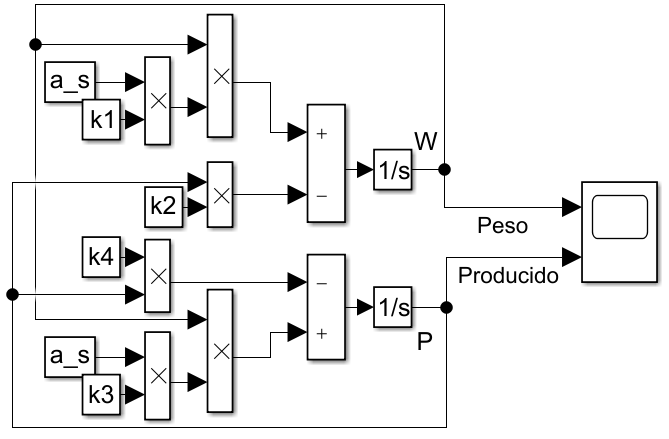
\includegraphics[scale=0.69]{img/simulinkwp1.png}
	 \end{center}
	 \caption{Diagrama de bloques del modelo EDO-WP en Matlab-Simulink. \label{modbloques}}
\end{figure}

\pagebreak
\subsubsection{Comportamiento del modelo EDO-WP en Simulink} \label{simulwp}

Dejando de lado los valores iniciales existentes para las variables en cuestión para cada una de las vacas mencionadas en la tabla \ref{Nporpartos}; como primera medida se considerarán valores promedios de $400[kg]$ y $40[kg]$ para el peso W y para la materia producida P respectivamente. Estos valores cumplirán su papel como valores iniciales en la simulación de este sistema que se asemeja al de un problema convencional de valor inicial.

Una vez establecidas los valores iniciales de los elementos integradores del sistema se procede a observar su comportamiento para distintos valores de $k_{i}$ con $i=1,2,3,4$. Los valores de $k_{i}$ aquí mostrados son netamente ejemplificativos.

\begin{itemize}
    \item \textbf{Escenario \#1 - $(k_{i}=1)$:} El resultado de las funciones W y P evidencian un crecimiento desde el valor inicial, hasta llegar a un punto de estabilización en donde el peso y la producción de materia orgánica es constante (ver figura \ref{igualkipng}). Esto no es sorpresa, pues el factor positivo que incrementa el peso es mayor que el factor negativo que  lo disminuye. Y teniendo en cuenta que la leche y heces producidas por el animal dependen de su peso, el comportamiento es más que justificado.
    
        \begin{figure}[H]
        	 \centering
        	 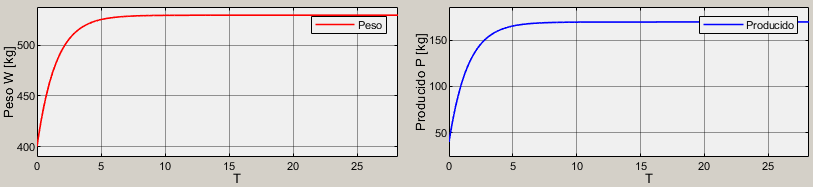
\includegraphics[scale=0.75]{img/igualki.png}
        	 \caption{Comportamiento del modelo con $(k_{i}=1)$, para todo $i$. \label{igualkipng}}
        \end{figure}
    
    \item \textbf{Escenario \#2 - $(k_{1}>k_{2})$ y $(k_{3}>k_{4})$ $\overset{Ej.}{\implies}$ $k_{1}=1$, $k_{2}=0.5$, $k_{3}=1$, $k_{4}=0.5$:} En esta ocasión, el resultado observado (ver figura \ref{k1Mk2_k3Mk4png}) es similar al anterior, no obstante el incremento presentado es mucho mayor al anterior puesto que la perdida de energía tanto en el peso como en la materia producida es mucho menor.

        \begin{figure}[H]
        	 \centering
        	 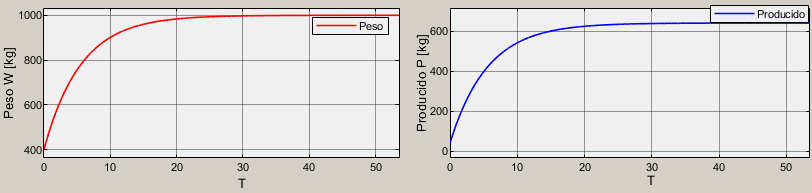
\includegraphics[scale=0.7750]{img/k1Mk2_k3Mk4.png}
        	 \caption{Comportamiento del modelo con $(k_{1}>k_{2})$ y $(k_{3}>k_{4})$. \label{k1Mk2_k3Mk4png}}
        \end{figure}
        
    \item \textbf{Escenario \#3 - $(k_{1}<k_{2})$, $(k_{3}<k_{4})$, $(k_{1}=k_{3})$ y $(k_{2}=k_{4})$ $\overset{Ej.}{\implies}$ $k_{1}=0.5$, $k_{2}=1$, $k_{3}=0.5$, $k_{4}=1$:} En esta ocasión, el resultado visual es similar al anterior, no obstante el incremento presentado en la figura \ref{k1menk2_k3menk4png} es mucho menor  para ambas variables y además, el tiempo que tarda en estabilizarse es mucho menor.

        \begin{figure}[H]
        	 \begin{center}
        	 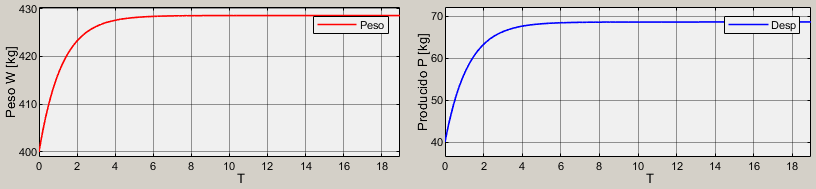
\includegraphics[scale=0.7750]{img/k1menk2_k3menk4.png}
        	 \end{center}
        	 \caption{Comportamiento del modelo con $(k_{1}<k_{2})$ y $(k_{3}<k_{4})$. \label{k1menk2_k3menk4png}}
        \end{figure}
        
    \item \textbf{Escenario \#4 - $(k_{1}<k_{3})$ y $(k_{2}<k_{4})$ $\overset{Ej.}{\implies}$ $k_{1}=0.6$, $k_{2}=0.69$, $k_{3}=0.65$, $k_{4}=0.8$:} Con esta simulación, se puede observar que el sistema se vuelve inestable (ver figura \ref{k1menk3_k2menk4png}), y tiende a crecer hacia el infinito. Si observamos detalladamente este escenario, si la tasa de conversión de energía del alimento hacia el producto de materia ($k_{3}$) es mayor que  que la tasa de conversión de energía del alimento hacia el peso ($k_{1}$) y además, la tasa de decrecimiento del peso ($k_{2}$) es menor que la tasa de decrecimiento de la materia producida ($k_{4}$); el peso total del animal irá incrementando más rápido de lo que decrece por procesos naturales, dando como resultado que el peso crezca indefinidamente.\\
    
    El crecimiento exponencial podrá verse afectado dependiendo de la diferencia en magnitud entre $k_{2}$ y $k_{4}$.
    
        \begin{figure}[H]
        	\centering
        	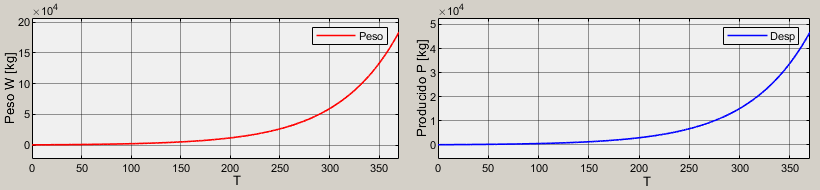
\includegraphics[scale=0.75]{img/k1menk3_k2menk4.png}
        	\caption{Comportamiento del modelo con $(k_{1}<k_{3})$ y $(k_{2}<k_{4})$. \label{k1menk3_k2menk4png}}
        \end{figure}
        
    \pagebreak
    \item \textbf{Escenario \#5 - $(k_{2} > k_{1})$ y $(k_{3}\gtrsim k_{4})$ $\overset{Ej.}{\implies}$ $k_{1}=0.1563$, $k_{2}=0.61$, $k_{3}=0.051755$, $k_{4}=0.0510$:} En esta ocasión se obtiene un resultado oscilante (ver figura \ref{k2Mk1_k3MAPk4png}), lo que quiere decir que el sistema presenta soluciones con parte imaginaria. Por tal motivo se puede establecer que debe existir una o varias restricciones entre los parámetros $k_{i}$.
    
        \begin{figure}[H]
            \centering
            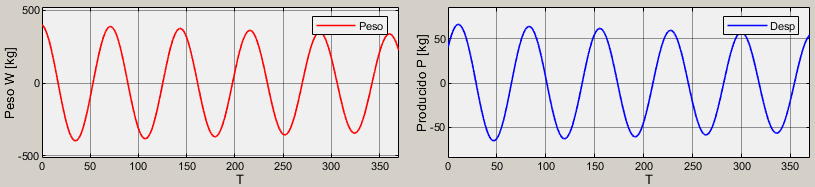
\includegraphics[scale=0.75]{img/k2Mk1_k3MAPk4.png}
            \caption{Comportamiento del modelo con $(k_{1}< k_{2})$ y $(k_{3}\gtrsim k_{4})$. \label{k2Mk1_k3MAPk4png}}
        \end{figure}
    
    Por un lado, es de esperar que si $(k_{2} > k_{1})$, significa que la primer ecuación diferencial tenderá a ser negativa y por lo tanto el peso W disminuirá. Por otro lado, al $(k_{3} > k_{4})$ es de esperarse que la producción de materia sea mayor que perdida de materia producida y por ende P aumentará. Con base en lo visto anteriormente, podemos establecer que se debe cumplir que $(|k_{1} - k_{2}| < k_{p})$. Siendo $|k_{p}|$ un valor pequeño que puede establecerse a futuro, pero que de momento sabemos no puede ser tal que $(k_{2} \approx 4*k_{1})$ o de lo contrario el sistema se indeterminará de mandera oscilante como el de la figura \ref{k2Mk1_k3MAPk4png}.
        
    \item \textbf{Escenario \#6 - $(k_{4}< k_{3})$ y $(k_{1}\gtrsim k_{2})$ $\overset{Ej.}{\implies}$ $k_{1}=0.051755$, $k_{2}=0.0510$, $k_{3}=0.61$, $k_{4}=0.051$:} En esta escenario también se obtiene un resultado oscilante (ver figura \ref{k3Mk4_k1MAPk2png}), lo que quiere decir que el sistema presenta soluciones con parte imaginaria. Por tal motivo se puede establecer que debe existir una o varias restricciones entre los parámetros $k_{i}$.\\

        \begin{figure}[H]
            \centering
            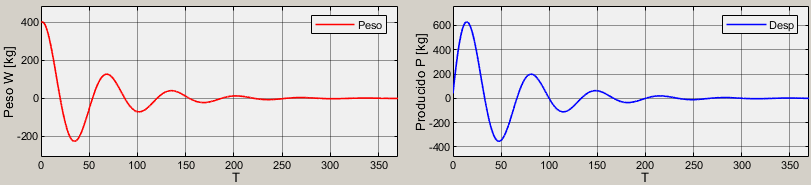
\includegraphics[scale=0.75]{img/k3Mk4_k1MAPk2.png}
            \caption{Comportamiento del modelo con $(k_{1}< k_{2})$ y $(k_{3}\gtrsim k_{4})$. \label{k3Mk4_k1MAPk2png}}
        \end{figure}
    
    Por un lado, estamos cumpliendo la restricción establecida en la situación anterior en donde $(k_{1} > k_{2})$. De esta manera podemos asegurar que la tasa de producción de peso W será mayor que la tasa de decrecimiento de peso por procesos naturales ($-k_{2}P$). Por otra parte, si $(k_{3} > k_{4})$, la producción de materia P será mayor que la materia perdida por procesos naturales ($-k_{4}P$) y por lo tanto $\dot{W}$ decaerá cuando la producción de materia sea muy alta. Cuando el peso disminuya hasta un valor matemáticamente negativo, y por ende la producción de leche y estiércol también lo hagan, la producción de estiércol será menor que la ganancia de peso y esto ocasionará un efecto oscilante tanto en el peso W como en la materia producida P hasta que se establezcan en un punto de equilibrio (W,P)=(0,0).
    
    Con base en las observaciones de esta situación y en las observaciones de los casos donde se inestabiliza el sistema por motive de $(k_{3} < k_{4})$ , podemos establecer que se debe cumplir que $(k_{3} \gtrsim k_{4})$ en pro de conseguir un punto medio antes que se inestabilice o se indetermine por soluciones matemáticamente imaginarias o complejas.
        
    \item \textbf{Escenario \#7 - $(k_{1}>k_{3})$ y $(k_{2}>k_{4})$ $\overset{Ej.}{\implies}$ $k_{1}=0.8$, $k_{2}=0.9$, $k_{3}=0.6$, $k_{4}=0.69$:} Llegados a este punto se sabe que $(k_{3} \gtrsim k_{4})$ y que $(|k_{1} - k_{2}| < k_{p})$, pero aún falta determinar las restricciones entre $(k_{1}$ y $k_{3})$ ,$k_{p}$ y $(k_{2}$ y $k_{4})$ . Teniendo en cuenta los valores de $k_{i}$ considerados en este escenario, se podría pensar que el resultado obtenido tendería a ser estable como el de la figura \ref{k1menk2_k3menk4png}, no obstante en esta situación se cumple que $k_{1} \neq k_{3}$ y $k_{2} \neq k_{4}$. 
    
            \begin{figure}[H]
        	 \centering
        	 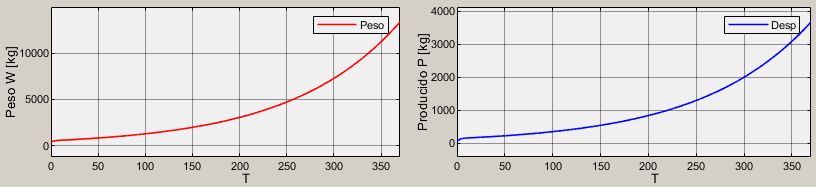
\includegraphics[scale=0.75]{img/k1Mk3_k2Mk4.png}
        	 \caption{Comportamiento del modelo con $(k_{1}>k_{3})$ y $(k_{2}>k_{4})$. \label{k1Mk3_k2Mk4png}}
        \end{figure}

    El resulta obtenido en la figura \ref{k1Mk3_k2Mk4png} evidencia que aún cuando el sistema tiende a estabilizarse en un valor determinado (cerca de T=15), el sistema rápidamente se indetermina hacia ordenes de magnitud alto. Por todo lo descrito en este y los escenarios anteriores podemos establecer que $(k_{2} > k_{4})$ sin que $(k_{2}$ sea muy grande comparado con $k_{4})$ (ver figura \ref{k2Mk1_k3MAPk4png}). Es decir que $(k_{2} \gtrsim k_{4})$.
    
    \item \textbf{Escenario \#8 - $(k_{1}\gtrsim k_{3})$, $(k_{2}\gtrsim k_{4})$ y $(k_{1}<k_{2})$ $\overset{Ej.}{\implies}$ $k_{1}=0.65$, $k_{2}=0.8$, $k_{3}=0.6$, $k_{4}=0.69$:} En este penúltimo escenario tenemos un resultado de la forma esperada, tanto para el peso W como para la materia producida P; en donde observamos un comportamiento creciente hasta que se estabiliza en un valor de referencia (que para el modelo es 0.0 en $T\approx 250$). No obstante, se observa que este comportamiento es logrado si se cumple que la diferencia absoluta entre $k_{1}$ y $k_{2}$ no sea mayor a 0.15. Esto es $(|k_{1} - k_{2}| < k_{p})$, con $|k_{p}| \leq 0.15$.
    
            \begin{figure}[H]
        	   \centering
        	   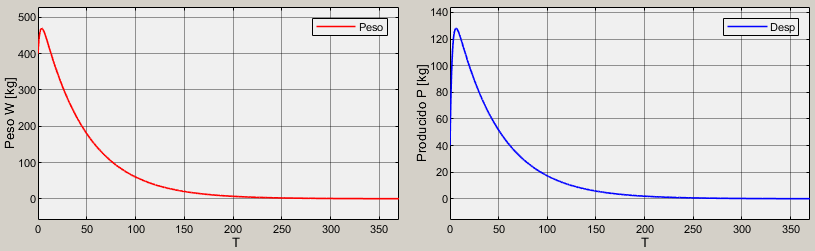
\includegraphics[scale=0.75]{img/k1MAPk3_k2MAPk4.png}
        	   \caption{Comportamiento del modelo con $(k_{1}\gtrsim k_{3})$ y $(k_{2}\gtrsim k_{4})$. \label{kiMAPpng}}
            \end{figure}

    \item \textbf{Escenario \#9 - $(k_{1}\gtrsim k_{3})$, $(k_{2}\gtrsim k_{4})$ y $(k_{1}\gtrsim k_{2})$ ($k_{p}\approx0.15$) $\overset{Ej.}{\implies}$ $k_{1}=0.95$, $k_{2}=0.8$, $k_{3}=0.9$, $k_{4}=0.69$:}  En este último escenario, nuevamente tenemos un resultado de la forma esperada; tanto para el peso W como para la materia producida P; en donde observamos un comportamiento creciente hasta que se estabiliza en un valor de referencia (que para el modelo es 0.0). A diferencia del caso anterior, se observa que el valor máximo para ambas variables, es mayor cuando $(k_{1}>k_{2})$ que cuando $(k_{1}<k_{2})$; mas sin embargo, el decrecimiento hasta el valor de estabilización es mucho más pronunciado ($T\approx 125$).
    
        \begin{figure}[H]
           \centering
           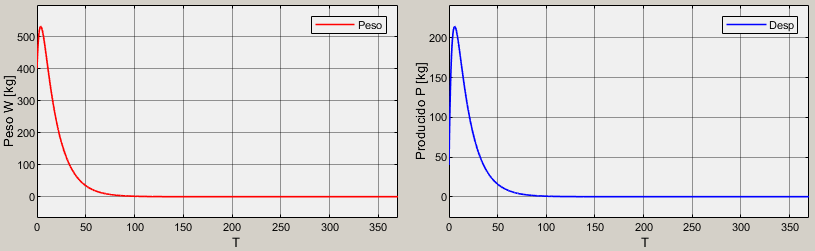
\includegraphics[scale=0.75]{img/k1MAPk3_k2MAPk4_k1Mk2.png}
           \caption{Comportamiento del modelo con $(k_{1}\gtrsim k_{3})$ y $(k_{2}\gtrsim k_{4})$. \label{kiMAPpng}}
        \end{figure}
            
\end{itemize}

Finalmente se puede llegar a la conclusión que el sistema de ecuaciones diferenciales ordinarias de dimensión 2 propuesto, puede prestarse para hallar soluciones numéricas de problemas de valor inicial para los datos existentes en este trabajo de grado. De esta forma, el modelo EDO-WP será usado para ajustar los datos existentes de Leche M, Estiercol E (Materia producida P) y Peso W; mediante optimización de parámetros por mínimos cuadrados.

\pagebreak
\subsection{Ajuste del modelo EDO-WP}\label{ajustemod}
% \subsection{Ajuste del modelo EDO-WP por mínimos cuadrados}

A partir del análisis descrito en la sección \ref{simulwp}, se puede afirmar que el sistema de ecuaciones diferenciales ordinarias de 2 dimensiones, está en la capacidad de ofrecer soluciones teóricas al problema de valor inicial y cuyas curvas presentan una forma similar a las previamente establecidas en la sección \ref{ajustenonlin}.
Ahora bien, los valores numéricos de los parámetros $k_{i}$ usados para ejemplificar los múltiples comportamientos del sistema de EDOs fueron valores usados para valores iniciales ficticios o artificiales tanto para el peso W como para la materia producida P. Por lo tanto, en pro de hallar los valores de los parámetros $k_{i}$ que corresponden a los registros de cada res y en cada parto, se debe hacer una ajuste del modelo a dichos datos. Este proceso requiere de un procesamiento de datos estructurados a manera de tablas o ``dataframes'' por lo que por facilidades algorítmicas se procede a implementar éste requerimiento mediante el lenguaje ``Python'', en el entorno de programación ``Anaconda - Jupyter Notebook'' teniendo en consideración la versatilidad que ofrecen ciertas librerías como ``numpy'' y ``pandas'' en cuanto a procesamiento de tablas de datos. Este proceso es descrito a continuación.

\subsubsection{Agrupación de datos para modelado}

Como se ha establecido en la sección \ref{ajustenonlin}, los registros existentes pueden variar en sus valores máximos, valores mínimos, formas de curva y duración o persistencia; dependiendo del parto del que hayan sido considerados para análisis. Adicionalmente, en la secciones \ref{reestructleche} y \ref{reestructpeso} se mencionó que los datos de leche M y peso W fueron reestructurados en forma de tablas de tal forma que se obtuvieran ``arrays'' de igual tamaño; y que posteriormente serían usados para ajustar los datos a modelos EDOs.\\

Por otra parte, en la sección \ref{dinamod} se mencionó que el estiércol producido sería considerado como un valor teórico y que éste presentaría una relación proporcional al peso entre un 1 y 10 por ciento del peso del animal, por lo que por efectos de simplificación en la complejidad de análisis; se ha consideraro que el estiércol producido E será aporximadamente un 5\% del registro de peso W. Por último pero no menos importante, en la sección \ref{dinamod} también se mencionó que el modelo EDO solo utilizaría 2 variables de estado en tanto que a diferencia del peso W, la leche y el estiércol eran consideradas como materia producida y que sería denominada como $P=M+E$ (ó $P=L+E$).\\

Pues bien, para ejemplificar el proceso algorítmico se utilizará el conjunto de datos que contiene la información de las reses pertenecientes al grupo de partos \#3 mas sin embargo este proceso se repite para todos y cada uno de los grupos de partos mencionados a lo largo de este trabajo de grado. En cuanto al proceso de implementación algorítmica secuencial, éste se describe a continuación:

\begin{enumerate}
    \item En primer lugar, se debe importar el conjunto de datos. Como se puede observar en la figura \ref{agrupmodpng}, cada res posee 3 columnas distintas que hacen referencia a cada una de las 3 variables iniciales W, M (ó L) y E. Adicionalmente, a diferencia de las columnas asociadas a los pesos de cada res, las columnas de leche y estiércol están separadas mediante un guión bajo ``$\_$'', distinción especialmente útil para agrupar columnas en el siguiente paso.
    
        \begin{figure}[H]
            \centering
            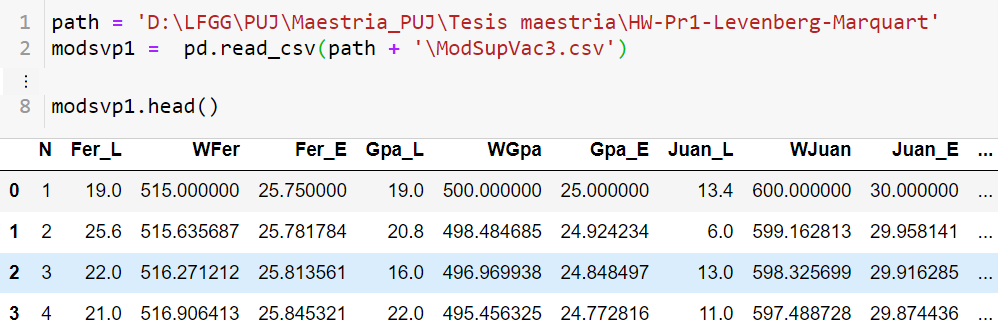
\includegraphics[width=\textwidth]{img/Agrupmod.png}
            \caption{Primeros 4 registros del conjunto de datos del grupo de parto \#3.}
            \label{agrupmodpng}
        \end{figure}

    \item En segundo lugar, sumamos las columnas de leche y estiércol, renombramos según corresponda y reorganizamos el conjunto de datos:

        \begin{figure}[H]
            \centering
            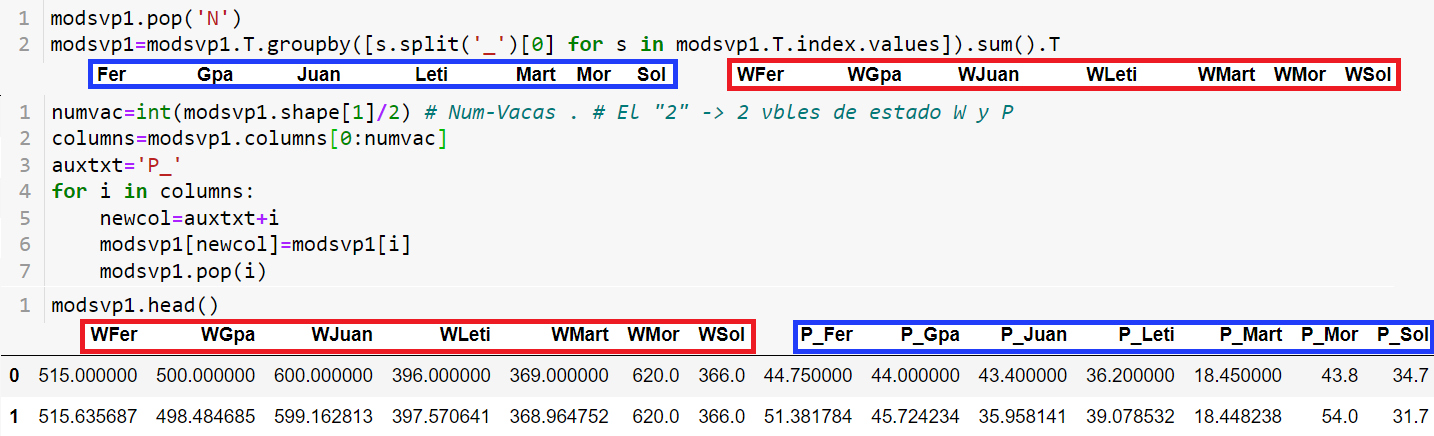
\includegraphics[width=\textwidth]{img/Agrupmod2d.png}
            \caption{Conjunto de datos del parto \#3 con solo 2 variables W y P para cada res.}
            \label{agrupmod2dpng}
        \end{figure}

    \item En tercer lugar, (en el lado izquierdo) separamos las variables de estado en matrices con los datos medidos correspondientes ($\mathcal{X}_1\_M=W$ y $\mathcal{X}_2\_M=P$); y (en el lado derecho)  consideramos los valores iniciales para cada res. Ver figura \ref{x1x2einitpng}

        \begin{figure}[H]
            \centering
            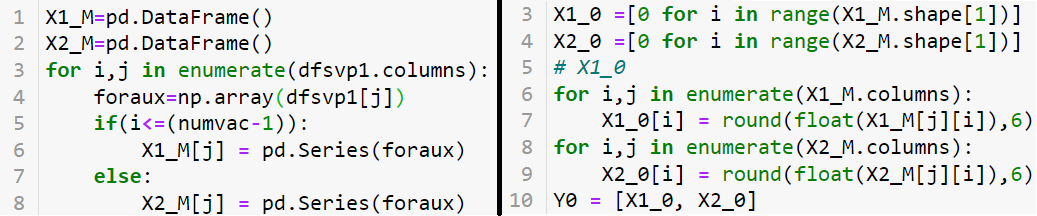
\includegraphics[scale = 0.56]{img/x1x2einit.png}
            \caption{Variables de estado W y P y sus respectivas condiciones iniciales, para cada res.}
            \label{x1x2einitpng}
        \end{figure}
\end{enumerate}

% \begin{figure}[H]
% 	 \begin{center}
% 	 \includegraphics[scale=0.64]{img/}
% 	 \end{center}
% 	 \caption{ \label{importmodelospng}}
% \end{figure}
\subsubsection{Optimización del ajuste del modelo por mínimos cuadrados} \label{optimizodeint}

        \begin{figure}[H]
            \centering
            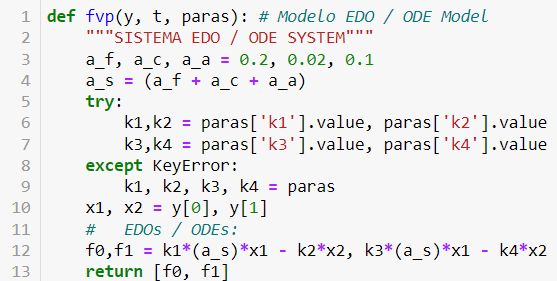
\includegraphics[scale=0.7]{img/modEDOpython.png}
            \caption{Modelo EDO-WP, implementación en Python.}
            \label{modEDOpythonpng}
        \end{figure}

\begin{enumerate} 
    \item En primer lugar, definimos las funciones del modelo (ver figura \ref{modEDOpythonpng}), el uso del solucionador ``odeint'' y el calculador de residuos; necesarias para resolver el modelo del tipo de problema de valor inicial (para más información, ver archivos ``ODE\_MOD WP\_Par$\#_{i}$'' del repositorio \cite{msclfggrepo}) y restringimos los parámetros del modelo (ver figura \ref{paramsaddpng}). Esto se realiza para cada una de las vacas mediante un bucle ``for''.
  
        \begin{figure}[H]
            \centering
            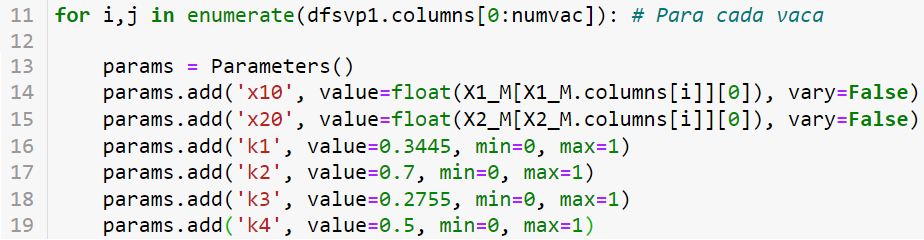
\includegraphics[width=\textwidth]{img/paramsadd.png}
            \caption{Restricciones del modelo EDO-WP implementado en Python.}
            \label{paramsaddpng}
        \end{figure}
        
    \item En segundo lugar, optimizamos el modelo propuesto en la sección \ref{dinamod} y repetimos para cada vaca mediante el mismo bucle ``for'' del paso anterior.
    
        \begin{figure}[H]
            \centering
            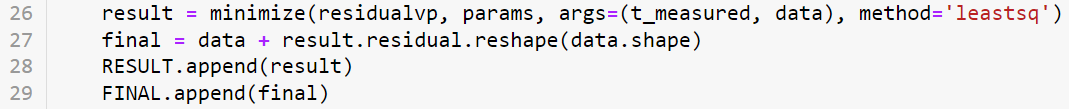
\includegraphics[width=\textwidth]{img/minimizefor.png}
            \caption{Soluciones de los modelos con ajuste de parámetros por mínimos cuadrados.}
            \label{paramsaddpng}
        \end{figure}
        
\end{enumerate}

\subsubsection{Visualización de resultados}

Tal y como se concluyó en la sección \ref{ajustemod} donde se estableció que el modelo EDO-WP podría ajustarse a los datos existentes referentes al peso W y a la materia producida P; es conveniente verificar si este ajuste ha sido logrado; por lo tanto procedamos a observar algunos de los resultados del ajuste del modelo.

Para ello analizaremos los resultados del ajuste a los datos de las reses del grupo de parto \#3:\\

\begin{itemize}
    \item \textbf{Fernanda (Fer)}\\
    
    Para este ejemplar, podemos observar en la figura \ref{ajustemodFerpng} que el la solución al modelo EDO-WP presenta un comportamiento creciente y luego decreciente, cuya forma  es similar a la que se quiere representar. Aún cuando visualmente podría considerarse que el ajuste no es lo suficientemente preciso, es importante resaltar que el ajuste por mínimos cuadrados ofrece errores relativos considerablemente bajos (ver valores de $k_{i}$ en la figura \ref{ajustemodFerstatspng}).
        \begin{figure}[H]
            \centering
            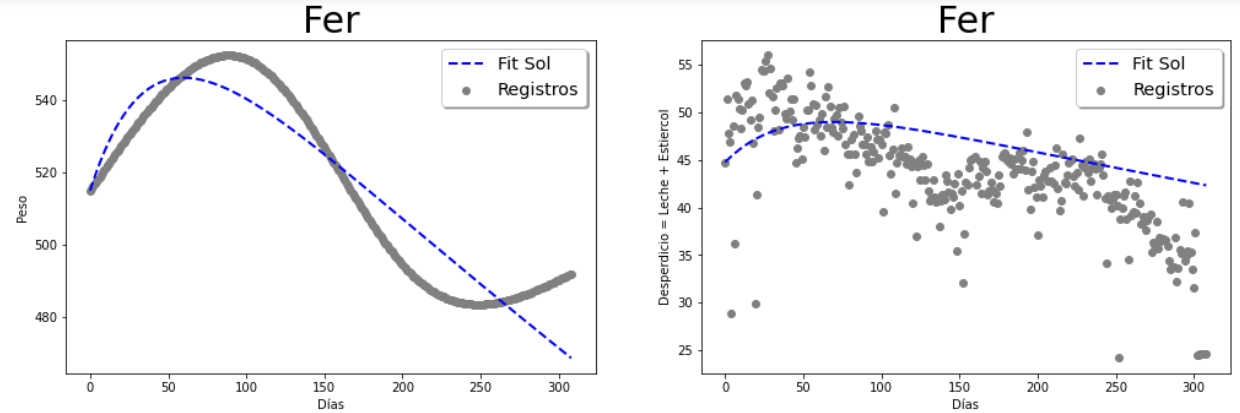
\includegraphics[scale=0.5]{img/ajustemodFer.png}
            \caption{Ajuste del modelo EDO-WP, a los datos de la res ``Fernanda''.}
            \label{ajustemodFerpng}
        \end{figure}
    Entre estos resultados podemos resaltar el hecho que el error relativo para cada uno de los parámetros $k_{i}$ es menor al 5\%.
        \begin{figure}[H]
            \centering
            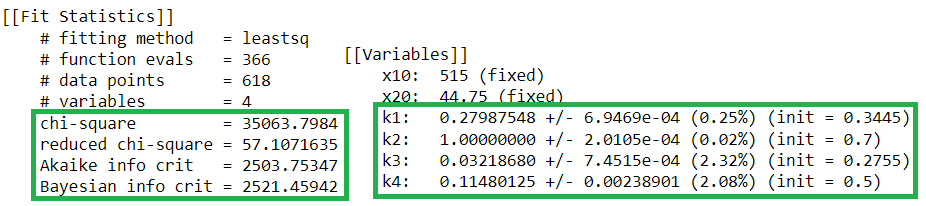
\includegraphics[scale=0.65]{img/ajustemodFerstats.png}
            \caption{Variables y datos estadísticos del ajuste.}
            \label{ajustemodFerstatspng}
        \end{figure}
        
    \pagebreak
    \item \textbf{Guapa (Gpa)}\\
    
    Con esta res podemos observar que el ajuste del modelo puede aproximar el comportamiento del peso respecto a su etapa decreciente y luego creciente, aún cuando el peso parece oscilar crecientemente alrededor de la solución planteada por el modelo (ver linea punteada en la figura \ref{ajustemodGpapng}). Con base en lo anterior se puede esperar que los parámetros $k_{1}$ y $k_{2}$ presenten errores considerablemente bajos. 
    \begin{figure}[H]
            \centering
            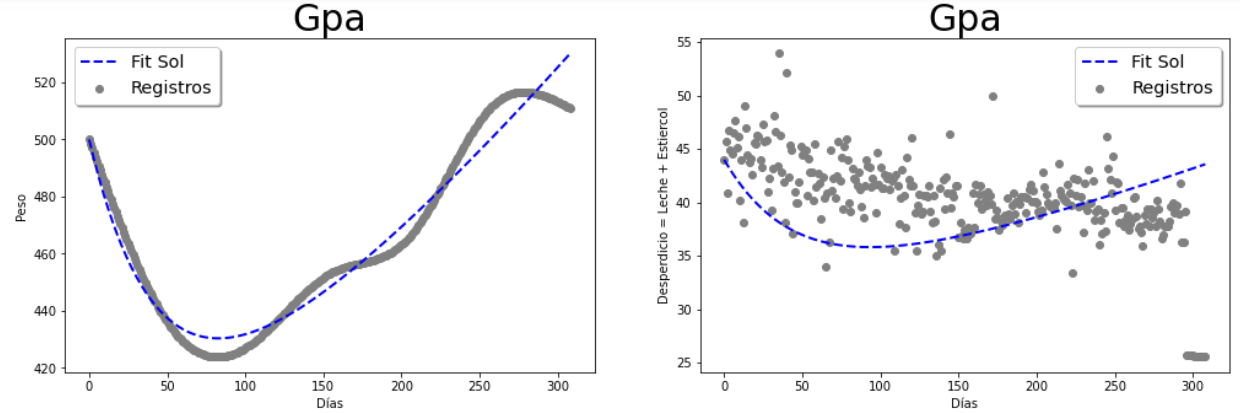
\includegraphics[scale=0.5]{img/ajustemodGpa.png}
            \caption{Ajuste del modelo EDO-WP, a los datos de la res ``Guapa''.}
            \label{ajustemodGpapng}
        \end{figure}
     A comparación del ajuste de modelo a la res Fernanda, los parámetros ajustados $k_{i}$ presentan un error relativo entre el 10\% y 16\% que podría interpretarse que el modelo no puede representar los datos de la variable P de manera satisfactoria. No obstante, también se puede pensar que el ajuste es relativamente mejor, puesto que por una parte el parámetro Chi cuadrado ($\chi^{2}$) reducido es más cercano a 1 que en el caso anterior, y por la otra parte los criterios AIC y BIC también presentan un valor menor; Estos valores reducidos comúnmente se entiende como un buen ajuste del modelo para los datos experimentales de la res en cuestión.
        \begin{figure}[H]
            \centering
            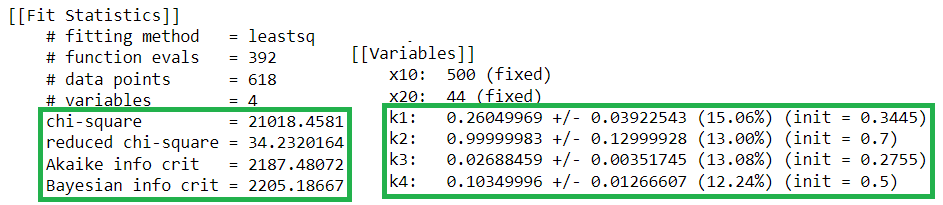
\includegraphics[scale=0.65]{img/ajustemodGpastats.png}
            \caption{Variables y datos estadísticos del ajuste.}
            \label{ajustemodGpastatspng}
        \end{figure}

    \pagebreak        
    \item \textbf{Juanita (Juan)}\\
    
    En cuanto a la vaca Juanita (ó Juan) se puede recalcar un ajuste similar al del caso anterior. Esto puede pensarse puesto que la solución del modelo EDO (linea punteada en la figura \ref{ajustemodJuanpng}) hace seguimiento del peso en su forma de onda con parte decreciente hasta aproximadamente los 150 días y su parte creciente hasta final del periodo de lactancia. En cuanto al seguimiento de la materia producida P se puede pensar que el modelo es fiel al comportamiento decreciente similar al que presentan los datos desde el valor máximo hasta los últimos registros cercanos al periodo de secado.
    
    Con base en lo anterior, se puede esperar que los parámetros $k_{i}$ hayan sido estimados con errores relativos considerablemente bajos. De manera general, se puede afirmar  que el modelo se ajusta relativamente bien para ambas variables, aunque con mejor fidelidad hacia el comportamiento decreciente del peso W que de la materia producida P. 
    
    \begin{figure}[H]
            \centering
            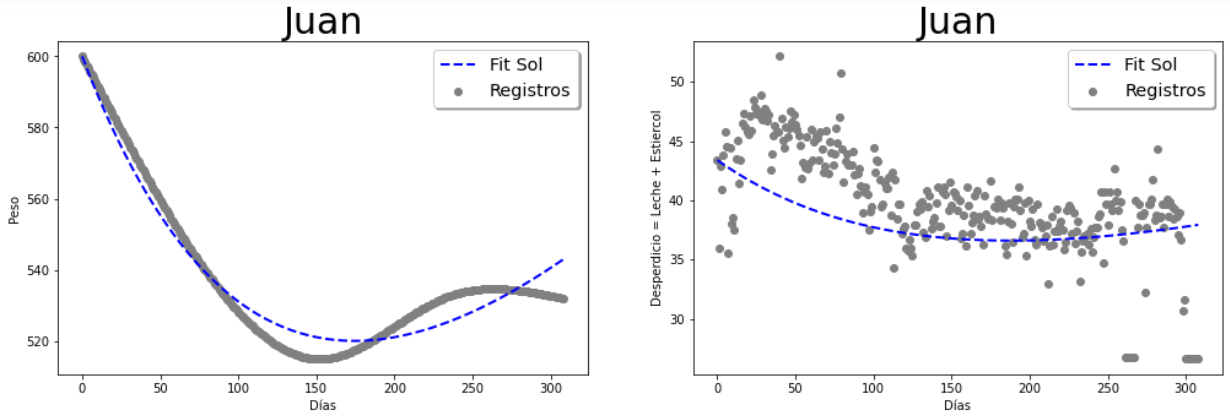
\includegraphics[scale=0.49]{img/ajustemodJuan.png}
            \caption{Ajuste del modelo EDO-WP, a los datos de la res ``Juanita''.}
            \label{ajustemodJuanpng}
        \end{figure}
    No obstante, aunque el ajuste del modelo no aparente ajustarse a los datos de la variable P, los datos de éste ejemplar han obtenido una minimización del error menor al 1\% además de presentar el menor valor de Chi cuadrado($\chi^{2}$)  reducido en comparación de todos los ajustes del grupo de partos \#3. Adicionalmente es importante mencionar que los criterios AIC y BIC disminuyen nuevamente en comparación del ajuste del modelo con los datos de la vaca Guapa.

        \begin{figure}[H]
            \centering
            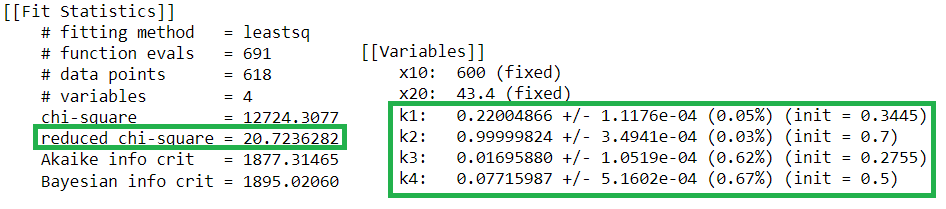
\includegraphics[scale=0.55]{img/ajustemodJuanstats.png}
            \caption{Variables y datos estadísticos del ajuste.}
            \label{ajustemodJuanstatspng}
        \end{figure}

    \item \textbf{Sol (Sol)}\\
    
    En esta ocasión tenemos un análisis interesante puesto que en esta ocasión el peso W es constante según se describió en la sección \ref{pocospesos}. Al asumir un peso constante en este periodo de lactancia debido a la falta de registros físicos o digitales de la res en cuestión, se esta limitando al modelo para que la primer ecuación del modelo EDO-WP sea aproximadamente 0 y por ende la ganancia de peso por la ingesta de alimento sea igual que la perdida de peso por procesos naturales. No obstante, para que esta afirmación se cumpla, se necesita que los parámetros $k_{1}$ y $k_{2}$ sean aproximadamente nulos, observación que claramente será notoria mediante un error de estimación alto; puesto que los valores usados como estimación inicial ($k_{1}=0.34$ y $k_{2}=0.7$) están muy alejados de los valores reales ($k_{1}=4.38e-10$ y $k_{2}=1.15e-10$) resultando en un error relativo considerablemente elevado con respecto a los valores de estimación inicial.. 
    
        \begin{figure}[H]
            \centering
            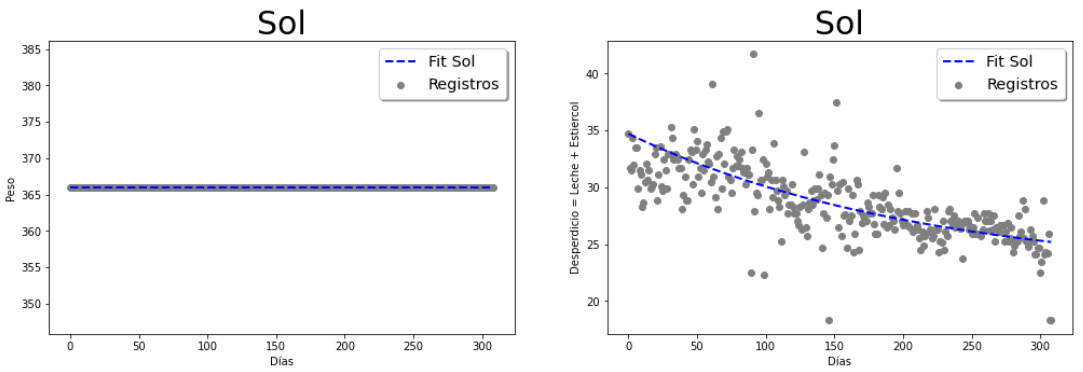
\includegraphics[scale=0.47]{img/ajustemodSol.png}
            \caption{Ajuste del modelo EDO-WP, a los datos de la res ``Sol''.}
            \label{ajustemodSolpng}
        \end{figure}

    Sin embargo, aún cuando el modelo no presente estimaciones iniciales cercanas para los primeros 2 parámetros, los resultados estadísticos generales si presuponen un buen ajuste del modelo a los datos del sujeto de estudio. Afirmación que puede soportarse con los valores de los errores relativos de los parámetros $k_{3}$ y $k_{4}$ menores al 20\% y a los valores más bajos de los criterios de Chi cuadrado ($\chi^{2}$) reducido, AIC y BIC. En cuanto al criterio ($\chi^{2}$), al ser el valor más cercano a 1 de todos los ajustes, se puede pensar que el grado de coincidencia entre las observaciones y las estimaciones es acorde con la varianza del error el ajuste.         

        \begin{figure}[H]
            \centering
            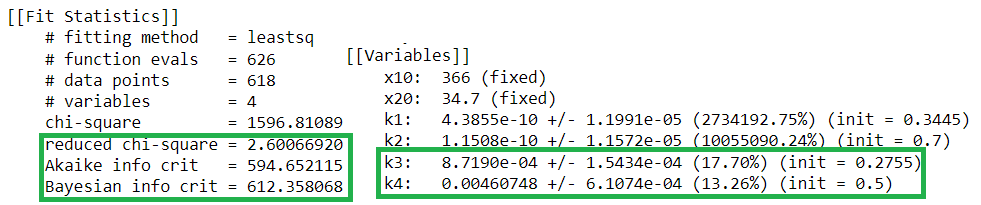
\includegraphics[scale=0.53]{img/ajustemodSolstats.png}
            \caption{Variables y datos estadísticos del ajuste.}
            \label{ajustemodSolstatspng}
        \end{figure}
        
        
    
    
\end{itemize}


% \textbf{Mostrar unas 2 gráficas buenas visualmente hablando y otras 2 gráficas que no ajusten bien y explicar porque... También hablar que la parte de comparación y/o evaluación de si el resultado es bueno o no se hará en el siguiente capitulo.}\\

% Mostrar las gráficas de los datos de leche, las gráficas de los datos de peso, las gráficas de los datos de estiércol, las gráficas netas de leche y estiércol. Mostrar los ajustes del modelo para cada parto y en las vacas en las que el error relativo es menor a 30\%

% \textit{\textbf{DEBERÍA MOSTRAR LOS OTROS EJEMPLARES EN DONDE EL AJUSTE FUE MALAS ? ? ? ? }}

% \pagebreak

% \subsection{Modelado por programación lineal entera} \label{linprogmod}
El proyecto en cuestión consiste en modelar dinámicamente la producción ganadera del CA-SENA-POP, en pro de predecir o estimar producciones futuras sin la necesidad de poseer los datos reales que corroborarían la precisión del modelo. Hasta ahora, los análisis propuestos requieren de un nivel avanzado de lenguajes de programación, álgebra lineal, ecuaciones diferenciales y estadística básica que pueden presentarse como una barrera al momento de presentar esta solución investigativa hacia los emprendedores ganaderos del centro agropecuario. Por tal motivo, se plantean los conjuntos, las variables, los parámetros y las funciones de objetivo de optimización mediante un ejercicio de optimización lineal que podría prestarse para maximizar ganancias o minimizar emisiones de $[KgCO_{2eq}]$. \\

En esta ocasión se plantea un problema de optimización lineal entera multipropósito, en donde la estimación de ganancia neta que presenta el CA-SENA-POP presenta un conflicto con la reducción de gases de $[KgCO_{2eq}]$, puesto que a mayor producción de estiércol, leche y carne; mayores son las emisiones de estos Gases de Efecto Invernadero (GEI).\\


% \section{Modelado por programación lineal entera} 
% Así pues, se plantea que:

% \subsubsection{Conjuntos}
% \begin{itemize}
% \begin{multicols}{2}
%     \item $VACAS_{v}$, indexadas por $v$
%     \item $DURACIONES_{d}$, indexadas por $d$
%     \item $PARTOS_{p}$, indexados por $p$
%     \item $DIAS_{t}$, indexados por $t$
%     % \item ESCENARIOS, indexados por $s$
% \end{multicols}
% \end{itemize}
% \subsubsection{Parámetros}

% \textbf{Emisiones de $[KgCO_{2eq}]$}

% \begin{itemize}
%     \item Según la ``Nicholas school of environment'' de la Universidad de Duke (\cite{ecoduke}), la producción de un (1) litro de leche representa una generación de  emisiones equivalentes de $Co_{2}$ de aproximadamente $1,39[KgCO_{2eq}/Lt_{leche}]$. Éstas emisiones son denominadas como ``GEIX''.
%     \item Según ``Statista.com'', una compañía de estadística comercial a nivel mundial (ver Referencia \cite{statista}), la producción de un (1) kilogramo de peso de ganado dedicado a la producción de leche, representa una generación de  emisiones equivalentes de $Co_{2}$ de aproximadamente $33,3[KgCO_{2eq}/Kg_{carne}]$. Éstas emisiones son denominadas como ``GEIY''.
%     \item Según \cite{manure}, la producción de un (1) kilogramo de estiércol representa una generación de  emisiones equivalentes de $Co_{2}$ de aproximadamente $0,0016108[KgCO_{2eq}/Kg_{estiercol}]$. Éstas emisiones son denominadas como ``GEIZ''.
% \end{itemize}
% % \subsubsection{Costos de producción}
% % \begin{itemize}
% %     \item Hasta donde sé el sena no me ha dado estos datos, probablemente no los tienen a la mano, entonces mejor no lo considero
% % \end{itemize}
% % \pagebreak

% \textbf{Precios de venta}

% \begin{itemize}
%     \item Según el CA-SENA-POP (ver Referencia \cite{casena}), el precio  de venta promedio de un (1) kilogramo de carne de res hembra (PVY) es de aproximadamente $7100[\$Pesos/Kg_{peso}]$. 
%     \item Según el CA-SENA-POP (ver Referencia \cite{casena}), el precio de venta de un (1) kilogramo de leche cruda sin análisis de proteína y grasas (PVX) es de aproximadamente $1350[\frac{\$Pesos}{Kg_{leche-cruda}}]$.
% \end{itemize}

% \textbf{Producción}

% \begin{itemize}
%     \item Según los registros proporcionados de manera física y digital del CA-SENA-POP (ver Referencia \cite{casena}), las producciones mínimas de leche pueden representarse como un parámetro $PMINX_{vp}$ en [$Kg_{leche}$/$Vaca_{v}Parto_{p}$]
%     \item Según los registros proporcionados de manera física y digital del CA-SENA-POP (ver Referencia \cite{casena}), las producciones mínimas de carne pueden representarse como un parámetro $PMINY_{vp}$ en [$Kg_{carne}$/$Vaca_{v}Parto_{p}$]
%     \item Según los registros proporcionados de manera física y digital del CA-SENA-POP (ver Referencia \cite{casena}), las producciones mínimas de estiércol pueden representarse como un parámetro $PMINZ_{vp}$ en [$Kg_{estiercol}$/$Vaca_{v}Parto_{p}$]
%     \item Según los registros proporcionados de manera física y digital del CA-SENA-POP (ver Referencia \cite{casena}), las producciones máximas de leche pueden representarse como un parámetro $PMAXX_{vp}$ en [$Kg_{leche}$/$Vaca_{v}Parto_{p}$]
%      \item Según los registros proporcionados de manera física y digital del CA-SENA-POP (ver Referencia \cite{casena}), las producciones máximas de carne pueden representarse como un parámetro $PMAXY_{vp}$ en [$Kg_{carne}$/$Vaca_{v}Parto_{p}$]
%       \item Según los registros proporcionados de manera física y digital del CA-SENA-POP (ver Referencia \cite{casena}), las producciones máximas de leche pueden representarse como un parámetro $PMAXZ_{vp}$ en [$Kg_{estiercol}$/$Vaca_{v}Parto_{p}$]
%     % \item Según el CA-SENA-POP (\cite{casena}), el precio de venta de un (1) kilogramo de leche cruda (PVKGLEC) es de aproximadamente $1350[\frac{\$Pesos}{Kg_{leche-cruda}}]$.
% \end{itemize}

% % \subsubsection{Variables}

% % \begin{itemize}
% %     \item   \begin{equation*}
% %                 \mathcal{X}_{ijdts}
% %             \end{equation*}
% % \end{itemize}

% \subsubsection{Variables}
% \begin{itemize}
%     \item \textbf{$\mathcal{X}_{vpdts}$} $\longrightarrow$ Cantidad de leche producida por una vaca $v$ en un grupo de parto $p$ que tiene una duración de lactancia aproximada $d$ en un día $t$; en [$Kg_{Leche}$]. $\left(\mathcal{X}_{vpdts}\geq 0 \right)$.
%     % \item \textbf{$\mathcal{X}_{vpdts}$}, Cantidad de leche producida por una vaca $v$ en un grupo de parto $p$ que tiene una duración de lactancia aproximada $d$ en un día $t$ en un escenario $s$; en [$Kg_{Leche}$].
%     % \begin{equation*}
%     %     \mathcal{X}_{ijdts}
%     % \end{equation*}
%     \item \textbf{$\mathcal{Y}_{vpdts}$}$\longrightarrow$ Cantidad de carne producido por una vaca $v$ en un grupo de parto $p$ que tiene una duración de lactancia aproximada $d$ en un día $t$; en [$Kg_{Carne}$].  $\left(\mathcal{Y}_{vpdts}\geq 0 \right)$.
%     % \item \textbf{$\mathcal{Y}_{vpdts}$}, Cantidad de carne producido por una vaca $v$ en un grupo de parto $p$ que tiene una duración de lactancia aproximada $d$ en un día $t$ en un escenario $s$; en [$Kg_{Carne}$].
%     % \begin{equation*}
%     %     \mathcal{Y}_{ijdts}
%     % \end{equation*}

%     \item \textbf{$\mathcal{Z}_{vpdts}$}$\longrightarrow$ Cantidad de estiércol producido por una vaca $v$ en un grupo de parto $p$ que tiene una duración de lactancia aproximada $d$ en un día $t$; en [$Kg_{Estiercol}$].  $\left(\mathcal{Z}_{vpdts}\geq 0 \right)$.
%     % \item \textbf{$\mathcal{Z}_{vpdts}$}, Cantidad de estiércol producido por una vaca $v$ en un grupo de parto $p$ que tiene una duración de lactancia aproximada $d$ en un día $t$ en un escenario $s$; en [$Kg_{Estiercol}$].
% \end{itemize}

% \subsubsection{Funciones objetivo}

% \textbf{Maximizar ganancias}

% Si nos centramos únicamente en plantear el modelo en pro de maximizar las ganancias sin importar el impacto ecológico que estas producciones puedan representar, se tiene un modelo lineal cuya función objetivo estará representada por la ecuación \ref{ecutil}. Es importante tener en cuenta que para este análisis no se tiene conocimiento de los costos operacionales del CA-SENA-POP, por lo que son considerados nulos para este caso.
% En una situación donde se tenga conocimiento de estos valores económicos, basta con substraer el costo operacional asociado a cada lactancia monitoreada que puede ser considerado como un parámetro $COPER_{vpdt}$ (si el costo es diario durante toda la lactancia) ó $COPER_{vp}$ (si el costo es total, resultado de todo el periodo de lactancia).

% \begin{equation}\label{ecutil}
% \begin{split}
%     Max(UTILIDADES) =\left(PVX\sum_{v,p,d,t}\mathcal{X}_{vpdt}\right) + \left(PVY\sum_{v,p,d,t}\mathcal{Y}_{vpdt} \right) - \sum_{v,p,d,t}COPER_{vpdt}
% \end{split}
% \end{equation}

% \textbf{Minimizar emisiones de gases de efecto invernadero GEI.}

% Si nos centramos únicamente en plantear el modelo en pro de minimizar las emisiones de GEI sin tener en consideración las posibles repercusiones financieras que estas producciones puedan representar, se tiene un modelo lineal cuya función objetivo estará representada por la siguiente ecuación:

% \begin{equation}\label{ecemis}
% \begin{split}
%     Min(EMISIONES) =\left( GEIX\sum_{v,p,d,t}\mathcal{X}_{vpdt}\right) + \left(GEIY\sum_{v,p,d,t}\mathcal{Y}_{vpdt}\right) + \left(GEIZ\sum_{v,p,d,t}\mathcal{Z}_{vpdt} \right)
% \end{split}
% \end{equation}
% % \subsubsection{Multi-objetivo: Ganancia máxima y emisiones mínimas}

% \subsubsection{Restricciones}

% \textbf{Producción mínima}

% \begin{itemize}
% \begin{multicols}{2}
%     \item \textbf{$\mathcal{X}_{vpdts}\geq PMINX_{vp}$} $\longrightarrow \forall v,p $
%     \item \textbf{$\mathcal{Z}_{vpdts}\geq PMINZ_{vp}$} $\longrightarrow \forall v,p $
%     \item \textbf{$\mathcal{Y}_{vpdts}\geq PMINY_{vp}$} $\longrightarrow \forall v,p $
%     \item $PMINX_{vp}$, $PMINY_{vp}$, $PMINZ_{vp}$, $\geq 0$
    
% \end{multicols}
% \end{itemize}

% \textbf{Producción máxima}

% \begin{itemize}
% \begin{multicols}{2}
%     \item \textbf{$\mathcal{X}_{vpdts}\leq PMAXX_{vp}$} $\longrightarrow \forall v,p $
%     \item \textbf{$\mathcal{Z}_{vpdts}\leq PMAXZ_{vp}$} $\longrightarrow \forall v,p$
%     \item \textbf{$\mathcal{Y}_{vpdts}\leq PMAXY_{vp}$} $\longrightarrow \forall v,p$
%     \item $PMAXX_{vp}$, $PMAXY_{vp}$, $PMAXZ_{vp}$, $\geq 0$
    
% \end{multicols}
% \end{itemize}
% % \subsubsection{}





